\documentclass[10pt]{beamer}


\mode<presentation> 
{
  \usetheme{Diku}
  \beamertemplatenavigationsymbolsempty
  \setbeamercovered{invisible}
%  \setbeamercovered{transparent}
}



% \mode<presentation> 
% { \usetheme[nat,dogma]{Frederiksberg} }

% \usepackage[danish]{babel}
\usepackage[latin1]{inputenc}
\usepackage{times}
\usepackage[T1]{fontenc}
\usepackage[english]{babel}
\usepackage{hyperref}
\usepackage{animate}
%\usepackage{multimedia}
\usepackage{francois-preamble}
\usepackage{multirow}

\usepackage{multirow}
%\usepackage{movie15}

\newcommand{\cc}{{c\!\!,}}
\newcommand{\degr}[1]{{{#1}^\circ}}

\title{Vision and Image Processing:\\ Correspondence analysis, Stereo, Stitching}

\author[S. Olsen] % (optional, use only with lots of authors)
{S�ren Olsen}

\institute[DIKU] % (optional, but mostly needed)
{
  Department of Computer Science\\
  University of Copenhagen
}

\date[2014-15 B2] % (optional, should be abbreviation of conference name)
% {Research Presentation, Diku 2006}


% Insert page numbers
\pagenumbering{arabic}
\setbeamertemplate{footline}{\hspace{5pt}\insertpagenumber\vspace{10pt}}



\definecolor{gold}{rgb}{0.95,0.83,0.0}
\definecolor{orange}{rgb}{0.95,0.7,0.0}
% \definecolor{backblue}{rgb}{0.93,0.94,0.99}
\definecolor{backblue}{rgb}{0.95,0.94,0.99}
\definecolor{darkgreen}{rgb}{0.0,0.30,0.0} 

\setbeamercolor*{background canvas}{bg=backblue} 



\newcommand{\myemph}[1]{{\color{blue}{#1}}}
\newcommand{\intrg}[1]{\int_{{#1}=-\infty}^\infty}
\newcommand{\intRR}{\int_{-\infty}^\infty}

\AtBeginSection[]
{
  \begin{frame}<beamer>{Outline}
    \tableofcontents[currentsection,currentsubsection]
  \end{frame}
}

\begin{document}
\maketitle

% would be cool with more images showing applications


%-------------------------------------------------------------------
%   Start slides
%-------------------------------------------------------------------



% 

% ----------------------------------------------------
% \begin{frame}
%  \frametitle{Stereo disparity}
%  \begin{center}
%    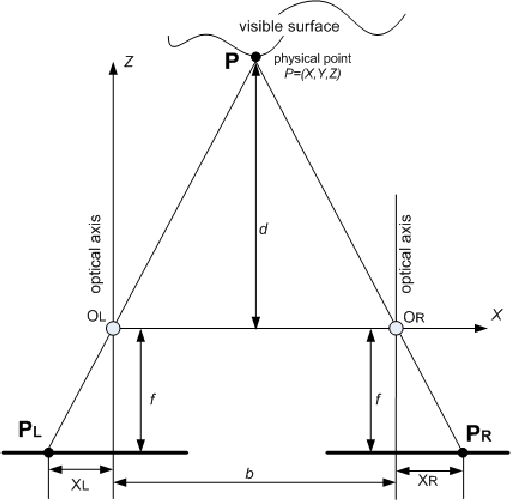
\includegraphics[width=0.9\textwidth]{MyImages/Stereo.png}
%   \end{center}
%  \begin{itemize}
%   \item Let the projection of $P$ on the baseline $O_L O_R$ be divided
%    in distances $A$ and $B$ and notice the two pairs of similar
%   triangles.
%  \item We have that $Z/A = f/x_L$ and that $Z/B = f/(-x_R)$.  Then
%    $$
%     b = A + B = Z \frac{x_L}{f} + Z \frac{-x_R}{f} = 
%    \frac{Z}{f} (x_L - x_R) = \frac{Z}{f}d
%    $$
%    where $d$ is the \myemph{disparity}.  Rewriting:
%   $$
%     Z = \frac{bf}{d}
%    $$
%   \end{itemize}
% \end{frame}


 


% ----------------------------------------------------
 \begin{frame}
   \frametitle{Geometric Calibration}
   \begin{itemize}
     \item Computing the camera matrix is called geometric calibration.
     \item Extrinsic parameters: (R,t): 
       Usually easy, but requires metric knowledge on scene features.
     \item Intrinsic parameters: (${\bf K}$): 
       Some parameters ($f$) are easy  and
       some ($(u_0, v_0)$) are difficult to estimate correctly.
   \end{itemize}
   \begin{columns}
     \column{0.5\textwidth}
     \begin{center}
       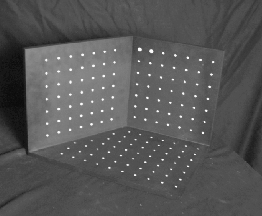
\includegraphics[width=0.8\textwidth]{../../VIP1415/Slides/IMAGES/calibrationobject}
     \end{center}
     \column{0.5\textwidth}
     \begin{itemize}
     \item Use an object with known geometry
     \item Use vanishing points / lines
     \item Use other cues...
     \end{itemize}
   \end{columns}
 \end{frame}


% Camera calibration ??? 

%----------------------------------------------
\begin{frame}
\frametitle{Repetition: The camera matrix}
Please recall the definition of the camera matrix:
\begin{displaymath}
      M =  K \left[ R \,\, {\bf t}\right]
\end{displaymath}
and the projection written out:
\begin{displaymath}
   w
   \begin{bmatrix}
     x\\y\\1
   \end{bmatrix}
   = \udesc{{\bf M}}{
      \udesc{{\bf K}}{
     \begin{pmatrix}
       f_x & 0 & u_0\\
       0 & f_y & v_0\\
       0 & 0 & 1
     \end{pmatrix}}
   \udesc{\left[{\bf R}\,\, {\bf t}\right]}{
     \begin{pmatrix}
       r_{11} & r_{12} & r_{13} & t_x\\
       r_{21} & r_{22} & r_{23} & t_y\\
       r_{31} & r_{32} & r_{33} & t_z\\
     \end{pmatrix}}}
   \begin{pmatrix}
     X\\Y\\Z\\1
   \end{pmatrix}
\end{displaymath}
or
\begin{displaymath}
   w
   \begin{bmatrix}
     x\\y\\1
   \end{bmatrix}
   =
     \begin{pmatrix}
       {\bf m}^1 \\
       {\bf m}^2 \\
       {\bf m}^3 \\
     \end{pmatrix}
   \begin{pmatrix}
     X\\Y\\Z\\1
   \end{pmatrix}
   =
     \begin{pmatrix}
       {\bf m}^1 U \\
       {\bf m}^2 U \\
       {\bf m}^3 U \\
     \end{pmatrix}
\end{displaymath}
where ${\bf m}^i$ is the $i$'th row of the camera matrix. 
\end{frame}






% ----------------------------------------------------
%  \begin{frame}
%   \begin{center}
%     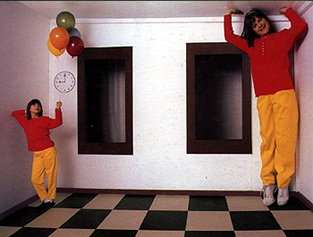
\includegraphics[width=0.8\textwidth]{../../VIP1415/Slides/IMAGES/amesroom}
%   \end{center}
%   Without knowledge of object geometry, calibration can be very problematic (Ames Room illusion).
% \end{frame}


% \section{More on Camera Models}

% ----------------------------------------------------
% \begin{frame}
%   \frametitle{Lens distortion}
%   Cheap or wide-angle lenses causes geometric lens distortion. The
%   most common distortion is (barral) radial distortion: 
%   \begin{center}
%   \begin{tabular}{c c c}
%     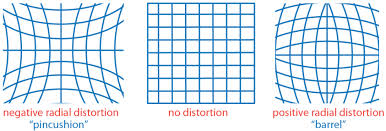
\includegraphics[width=0.55\textwidth]{../../VIP1415/Slides/MyImages/lensdistortion1.jpg}
%     & \hspace{2mm} &
%     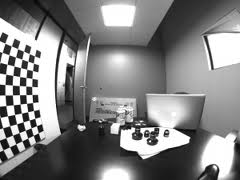
\includegraphics[width=0.3\textwidth]{../../VIP1415/Slides/MyImages/lensdistortion2.jpg}
%    \end{tabular}
%   \end{center}
%   To comply with the assumptions of the pin-hole camera it may be
%   necessary to correct for lens distortion before doing anything else.
% XS\end{frame}


% ----------------------------------------------------
% \begin{frame}
% \frametitle{Lens distortion}
% Lens distortion is non-linear.  The displacement of pixels may (for
% radial distortion) be modeled as multiplicative even ordered
% polynomium in radial distance from the principal point. \\[3mm]
%
%% \begin{tabular}{r r}
%%  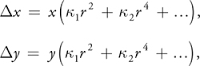
\includegraphics[width=0.5\textwidth]{../../VIP1415/Slides/lensdistortion4.png}

% \begin{minipage}{0.49\textwidth}
%    \begin{eqnarray*}
%      \Delta x  &=& x_r \left ( 
%             \kappa_1 r^2 \;+\; \kappa_2 r^4 \;+\; \cdots \right ) \\
%      \Delta y &=&  y_r \left ( 
%             \kappa_1 r^2 \;+\; \kappa_2 r^4 \;+\; \cdots \right ) \\
%      r^2  &= & x_r^2 + y_r^2 \\
%      x_r  &= & x - u_0 \\
%      y_r  &= & y - v_0 
%      \end{eqnarray*}
%\end{minipage}
%% \hspace{2mm}
% \begin{minipage}{0.50\textwidth}
%     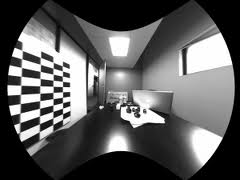
\includegraphics[width=0.50\textwidth]{../../VIP1415/Slides/MyImages/lensdistortion3.jpg}
% \end{minipage}
%%   \end{tabular}
%%  \end{center}
% \vspace{3mm}
%
% Often only one or two terms are used.  The two konstants $\kappa_1$
% and $\kappa_2$ are estimated using an iterative (nonlinear)
% optimisation approach.  
% \end{frame}


% ----------------------------------------------------
% begin{frame}
%   \frametitle{Shrinking the aperture}
%   \begin{center}
%    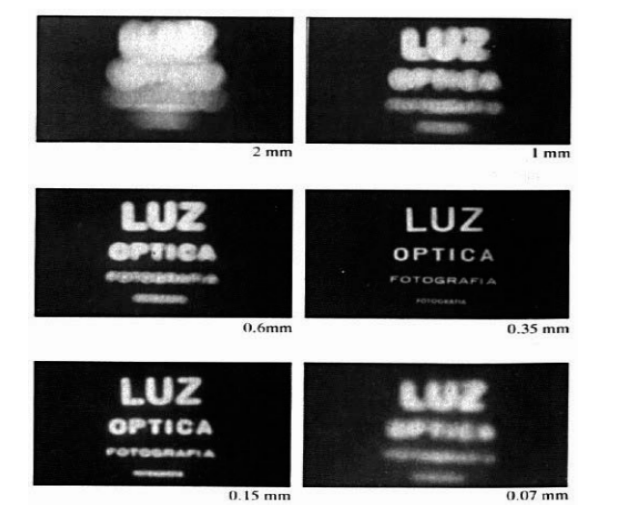
\includegraphics[width=0.7\textwidth]{../../VIP1415/Slides/IMAGES/shrinkingaperture}
%  \end{center}
%  Less light in, diffraction. 
% \end{frame}


% ----------------------------------------------------
% \begin{frame}
%   \frametitle{Focal Length, Aperture}
%   \begin{center}
%     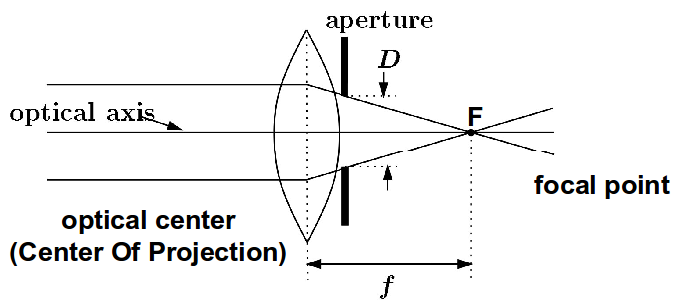
\includegraphics[width=0.8\textwidth]{../../VIP1415/Slides/FIGURES/focallength}
%   \end{center}
%   \begin{itemize}
%   \item Lens focuses parallel rays into a single point.
%   \item Aperture restricts range of rays.
%   \item Zoom by increasing $f$, make wide angle by decreasing $f$
%   \item In practice zoom optics use a set of lenses moving in a
%     non-linear way wrt. each other.
%   \end{itemize}
% \end{frame}


% ----------------------------------------------------
% \begin{frame}
%   \frametitle{Focus, Depth of Field}
%    \begin{center}
%     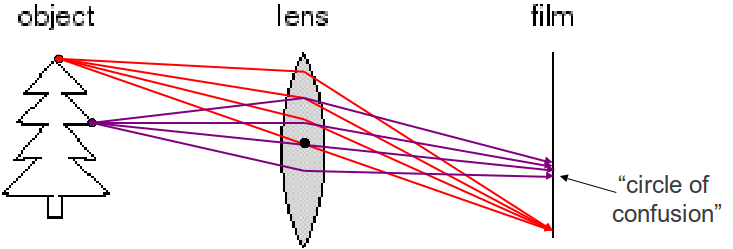
\includegraphics[width=0.7\textwidth]{../../VIP1415/Slides/FIGURES/addinglens}
%   \end{center}
%   \begin{itemize}
%   \item Specific distance for which objects are in focus
%   \item Changing shape of lens changes the focus distance.
%   \item Changing distance between lens and sensor changes the 3D
%     points in focus.
%   \end{itemize}
% \end{frame}


% ----------------------------------------------------
% \begin{frame}
%   \frametitle{The Eye is a Camera with Lens}
%     \begin{center}
%     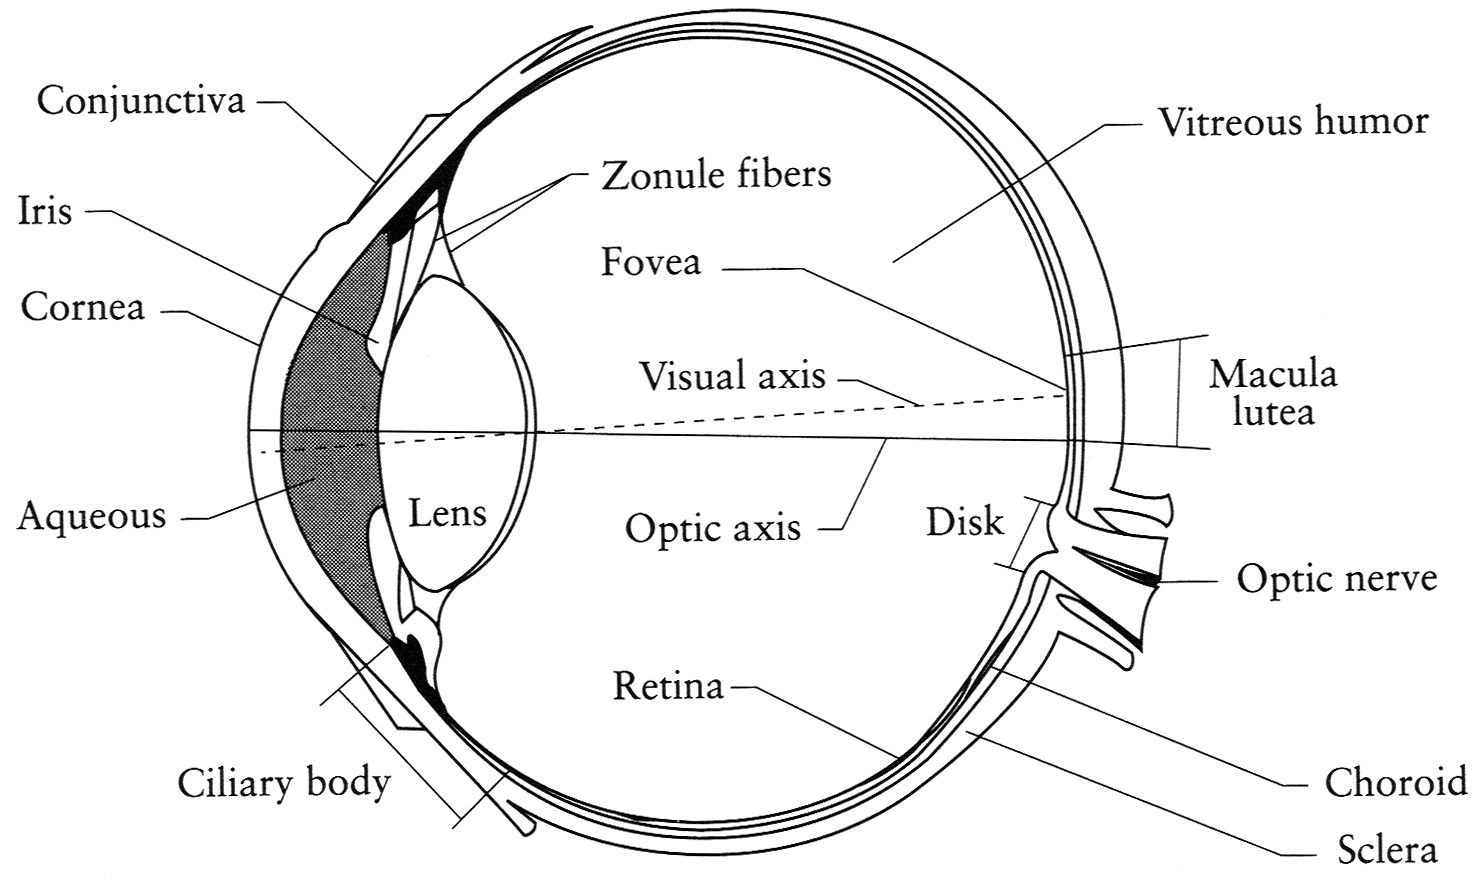
\includegraphics[width=0.9\textwidth]{../../VIP1415/Slides/FIGURES/theeye}
%   \end{center}
% \end{frame}


% ----------------------------------------------------
% \begin{frame}
%  \frametitle{Depth of Field}
%  \begin{center}
%    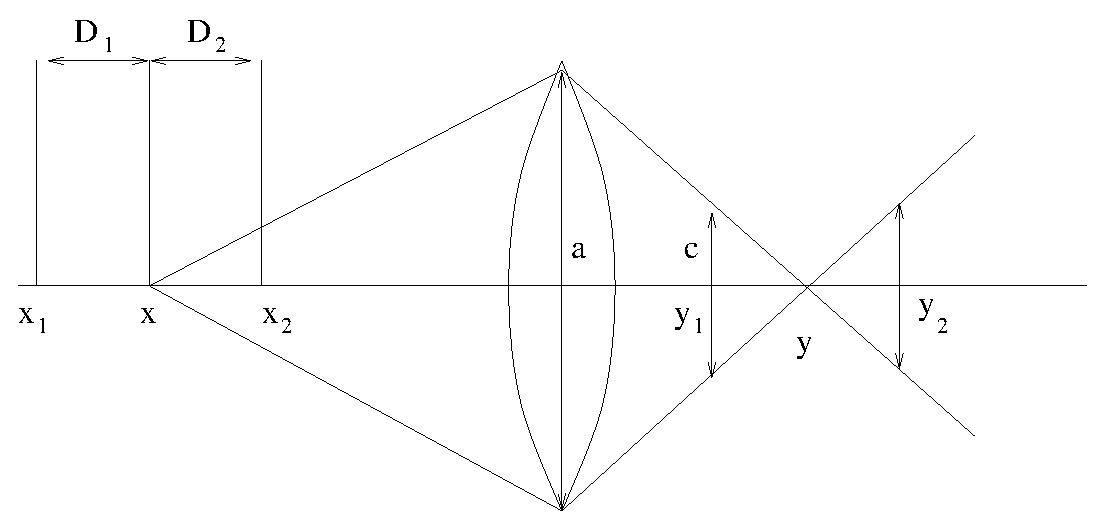
\includegraphics[width=0.6\textwidth]{../../VIP1415/Slides/FIGURES/depthoffield}
%  \end{center}
%  We shall later se that the Depth of field (DOF) is given by:
%  $$
%  DOF = \frac{2acfx(x-f)}{a^2f^2 - c^2x^2} \approx \frac{2cx^2}{af}
%  $$
%  where $a$ is the aperture, $f$ is the focal length, $c$ is the pixel
%  diameter, and $x$ is the distance. 
%  \begin{itemize}
%    \item To have a large DOF we would like large $c$ and $x$ and
%      small values of $f$ and $a$.
%    \item To estimate depth from focus we want a small DOF
%  \end{itemize}
%\end{frame}


% ----------------------------------------------------
% \begin{frame}
%  \frametitle{Depth from focus}
%  % \begin{center}
%    % 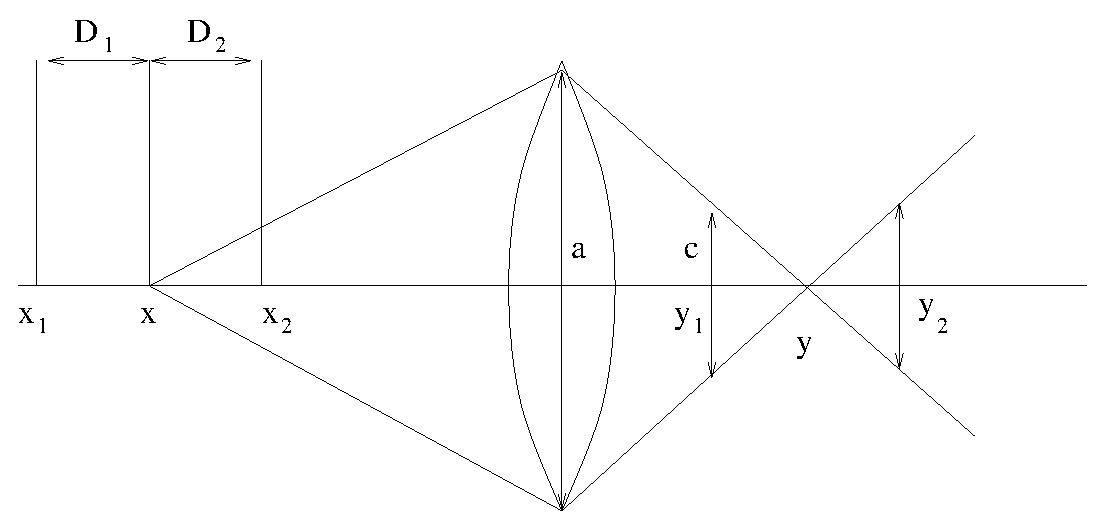
\includegraphics[width=0.9\textwidth]{../../VIP1415/Slides/FIGURES/depthoffield}
%  % \end{center}
%  A more realistic cemara model than the pin-hole model is the {\em
%    thin-lens} model. We shall later show that the equation for such a
%  lens is:
%  $$
%  \frac{1}{Z} + \frac{1}{d} = \frac{1}{f} 
%   \hspace{10mm}\mbox{or} \hspace{10mm}
%   Z  = \frac{fd}{d - f} 
%  $$  
%  where $f$ is the focal length and $d$ is the distance between the
%  lens and the image plane. 
%   \medskip
%
%  Thus, depth may be recovered from
%  knowledge of the focus setting that  brings things into focus. More
%  about this and Depth of field in a later lecture.
% \end{frame}


% ----------------------------------------------------
\begin{frame}
\frametitle{What can we see with two eyes}
    \begin{center}
      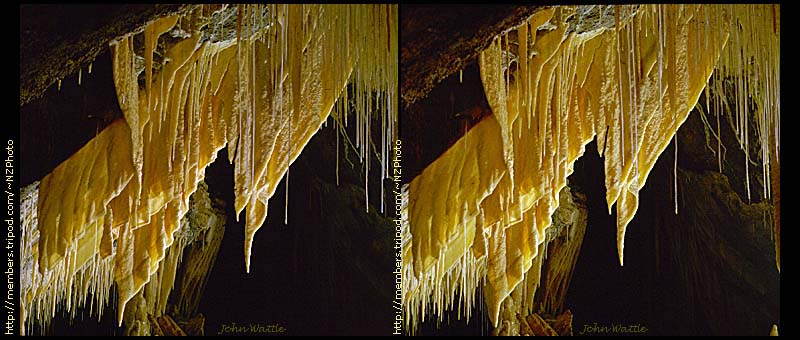
\includegraphics[width=0.9\textwidth]{../../VIP1415/Slides/MyImages/stereoEX1.jpg}
  \end{center}
Stereo vision is among the most important human sensing methods.
\medskip
Next lecture we will talk a lot about stereo vision.
\end{frame}


% ============================================
% Correspondences from 2018/19
% ----------------------------------
% \section{Stereo Vision}


\begin{frame}
  \frametitle{Multiple View Correspondences}
  \begin{center}
    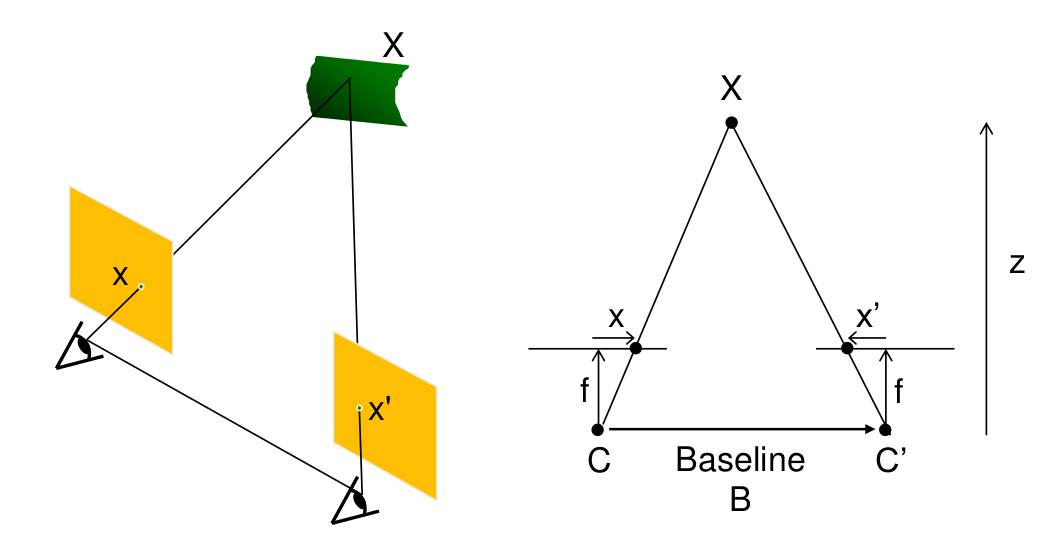
\includegraphics[width=0.9\textwidth]{../../VIP1516/lectures/FIGURE/stereo}
  \end{center}
  If we can recover $x'$ from $x$ we can recover depth: $z = - \frac{fB}{x'-x}$.
\end{frame}



%---------------------------------------------
% \begin{frame}
%   \frametitle{Image Correspondence}
%   \begin{center}
%     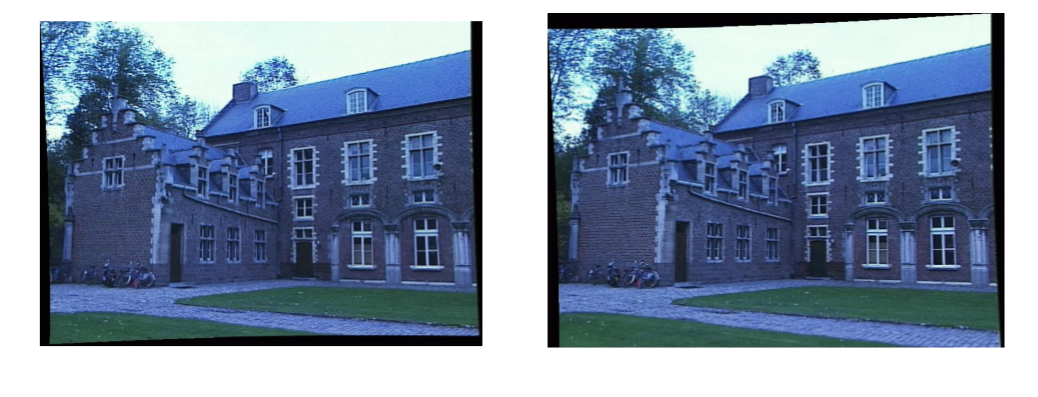
\includegraphics[width=0.9\textwidth]{../../VIP1516/lectures/IMAGES/stereo2images}
%   \end{center}
%   How do we match points from image 1 to image 2: You should have seen
%   some of it before,  but this is not the end of the story!
% \end{frame}




%---------------------------------------------
\begin{frame}
  \frametitle{Epipolar Constraints}
  \begin{center}
    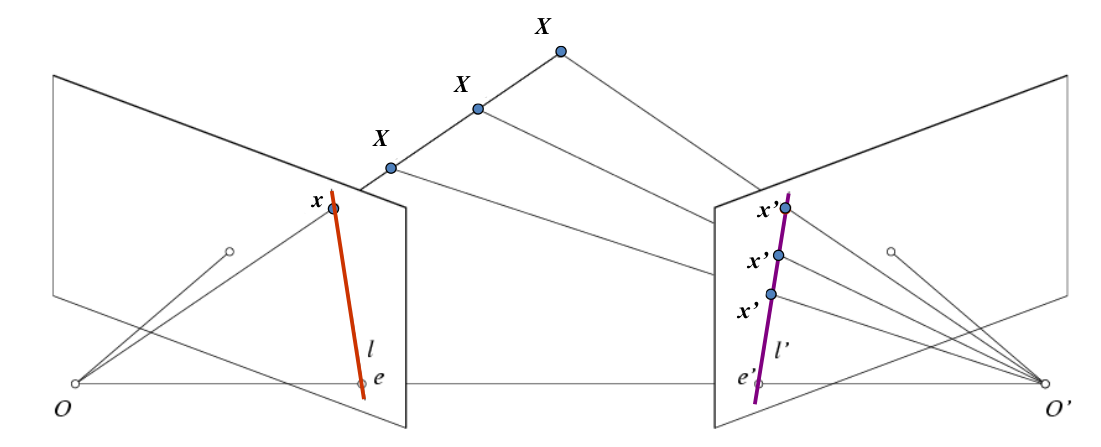
\includegraphics[width=0.9\textwidth]{../../VIP1516/lectures/FIGURE/epipolarconstraint}
  \end{center}
  \begin{itemize}
  \item  Corresponding point for $x$ must lie in corresponding line $l'$
  \item  Corresponding point for $x'$ must lie in corresponding line $l$
  \end{itemize}  
\end{frame}



%----------------------------------------------
% \begin{frame}
%   \frametitle{Epipolar Constraints}
%   \begin{center}
%     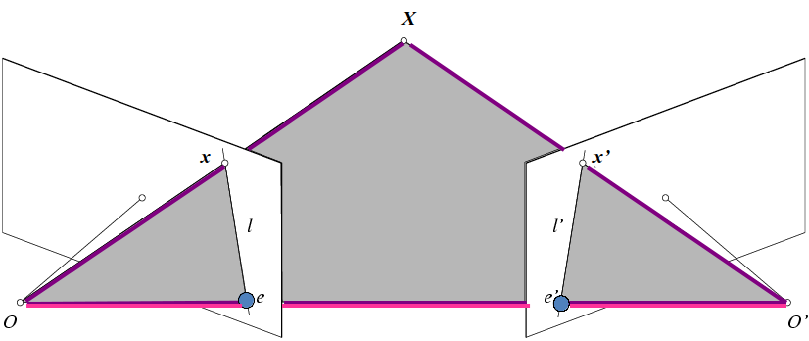
\includegraphics[width=0.9\textwidth]{../../VIP1516/lectures/FIGURE/epigeom}
%   \end{center}
%   \begin{itemize}
%   \item  Line connecting $O$ and $O'$: \myemph{baseline}
%   \item Plane through baseline and $x$ or $x'$: \myemph{Epipolar Plane}
%   \item Epipoles: intersection of baseline and image planes:
%     projection of the other camera center.
%   \item Epipolar Lines - intersections of epipolar plane with image
%     planes (always come in corresponding pairs)
%   \end{itemize}  
% \end{frame}


%----------------------------------------------
\begin{frame}
  \frametitle{Example: Converging cameras}
  \begin{center}
     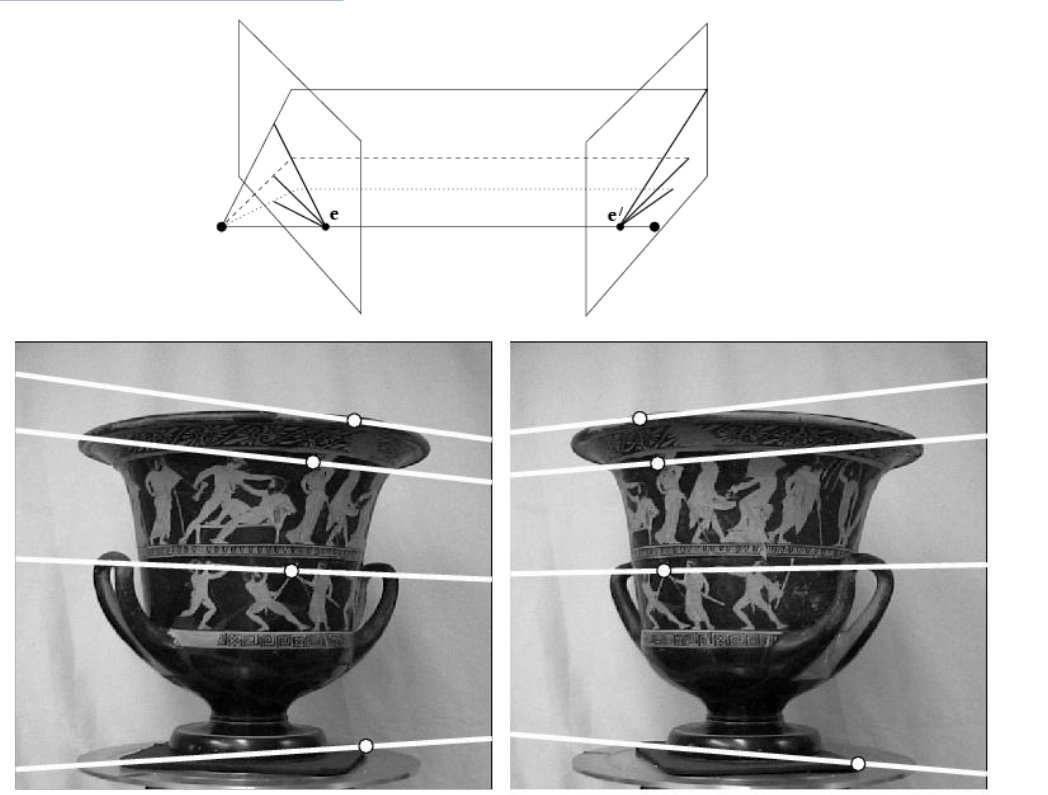
\includegraphics[width=0.9\textwidth]{../../VIP1516/lectures/FIGURE/convergecam}
  \end{center}
\end{frame}



%----------------------------------------------
\begin{frame}
  \frametitle{Calibrated Case}
   \begin{center}
    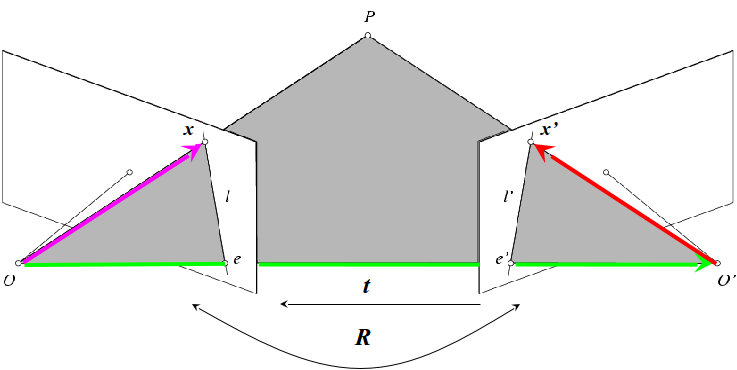
\includegraphics[width=0.65\textwidth]{../../VIP1516/lectures/FIGURE/epicalibrated}
  \end{center}
  Camera parameters known for the two cameras: calibration matrices $K$ and $K'$\\
\end{frame}



%----------------------------------------------
% \begin{frame}
%    \frametitle{The essential matrix $E$}
%   \begin{itemize}
%   \item  Let $y$ and $y'$ be 3D coordinates of the same scene point in
%     the two (different) 3D-{\bf camera} coordinate systems. The two
%    systems are related by a rotation and a translation. \\[3mm]
%     $$y' = R(y-\bt)$$
%   \item We will later show that corresponding points $y_c$ and $y'_c$
%     are related by a $3 \times 3$ matrix $E$ built from $R$ and $t$  \\[3mm]
%     $$
%     y_c^T E y'_c = 0.
%     $$
%   \item $E$ is called the \myemph{essential matrix} (Longuet-Higgins
%     1981).
%   \end{itemize}
% \end{frame}



%----------------------------------------------
% \begin{frame}
%    \frametitle{The fundamental matrix $F$}
%   \begin{itemize}
%     \item For corresponding points, the image coordinates ($x$ and
%       $x'$) are related to the camera coordinates ($y$ and $y'$)
%      through the calibration matrices $K$ and $K'$. Thus: 
%       $$
%           0 = y^T E y' = (K^{-1} x)^T E (K'^{-1} x') = 
%           x^T (K^{-T} E K'^{-1} ) x' = x^T F x'
%       $$
%       where $x$ and $x'$ are the homogene representation of the
%       corresponding points in image coordinates, and where $F$ is the
%       \myemph{fundamental matrix}. \\[3mm]
%   \item Given a sufficient number of corresponding image points ($x$ and $x'$),
%     the fundamental matrix $F$ can be estimated.
%   \item Given the internal intrinsic parameters ($K$ and $K'$) the
%     essential matrix $E$ may be computed from $F$.
%   \item Given $E$, the position and orientation of camera 1 vs camera
%     2 (i.e., $R$ and $\bt$) can be recovered. 
%   \end{itemize}
% \end{frame}
 




%----------------------------------------------
\begin{frame}
  \frametitle{The Fundamental matrix}
  Ther fundamental matrix is a $3 \times 3$ matrix that relates
  corresponding points in a bilinear homogeneous equation:

  \begin{displaymath}
    \left [ x_L, \;y_L,\; 1 \right ] \; F \;
    \left [ \begin{array}{c}
              x_R \\ y_R \\ 1
            \end{array}              
          \right ] \;\; = \;\; 0 
  \end{displaymath}

  $F$ has 9 elements, but it can be shown that $\det F = 0$, so it has
  only 7 degrees of freedom (independent parameters). \\[3mm]

  Fixing either the left or right image point gives a straight line
  (the epipolar line) in the other image.
  
 \end{frame}
 




%----------------------------------------------
\begin{frame}
   \frametitle{Calibration and reconstruction}
   \begin{itemize}
     \item Given (sufficient) image point correspondences, the
       fundamental matrix $F$ may be estimated
       using linear algebra. \\[4mm]
     \item Linear estimation of $F$   is easy, but not accurate. In
       practice a non-linear post- non-linear optimisation is needed. \\[4mm]
      \item Given $F$, the stereo correspondence problem is reduced
        to a one-dimensional search along the epipolar lines. \\[4mm]
      \item Given $F$, and the internal camera parmeters $K$ and $K'$,
        then the reconstructions of 3D points is possible (using
        linear algebra) from image point correspondences.
      \end{itemize}
      \bigskip

      If you want to know more, you must take the ATIA-course.
\end{frame}




%----------------------------------------------
% \begin{frame}
% \frametitle{Proof of $x_R^{\top}Ex_L = 0$}
% \begin{center}
%       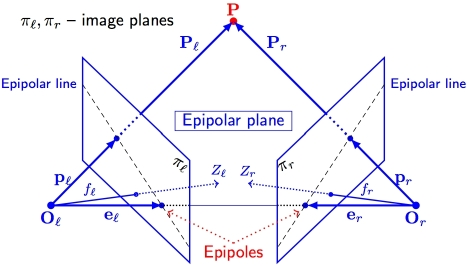
\includegraphics[width=0.7\textwidth]{../../VIP1516/lectures/MyImages/epipolarGeom.jpg}
% \end{center}
% We have that the camera coordinate systems are related by:
% \begin{displaymath}
%    {\bf P}_R = R ( {\bf P}_L - {\bf T})
% \end{displaymath}
% 
% \begin{definition}
%   The coplanarity condition:  
%   ${\bf P}_L$, ${\bf T}$, and 
%   ${\bf P}_L - {\bf T}$ are all in the epipolar plane. Then, also
%    $R^{\top}{\bf P}_R$  is within the plane.
% \end{definition}
% \end{frame}



%----------------------------------------------
% \begin{frame}
% \frametitle{The cross-product}
% The cross-product between two vectors ${\bf a}$ and ${\bf b}$ is a
% vector that is perpendicular to both:
%
% \begin{displaymath}
%    {\bf a} \times {\bf b} \;=\; 
%    \left ( 
%    \begin{array}{c}
%    -a_3 b_2 + a_2 b_3 \\ a_3 b_1 - a_1 b_3 \\ -a_2 b_1 + a_1 b_2
%     \end{array}
%     \right )
%     \;=\; S {\bf b}
% \end{displaymath}
% where \\[3mm]
% \begin{displaymath}
%    S \;=\; [a]_x \;=\; \left [
%      \begin{array}{c c c}
%         0    & - a_3 & a_2  \\ 
%         a_3 &    0    & -a_1 \\
%       -a_2 &  a_1   &  0
%      \end{array}
%    \right ]
% \end{displaymath}
% 
% $\mbox{}$ \\[2mm]
% We see that $S$ is an anti-symmetric and rank deficient matrix. $S$
% has rank 2.
% \end{frame}



%----------------------------------------------
% \begin{frame}
%  \frametitle{Proof cont. 2}
% Because  ${\bf P}_L$, ${\bf T}$, and ${\bf P}_L - {\bf T}$ all are in
% the epipolar plane we can write:\\[3mm]
%
% \begin{eqnarray*}
%  0 & = &   ({\bf P}_L - {\bf T}) ^{\top} {\bf T} \times {\bf P}_L \\[2mm]
%     & = &  (R^{\top}{\bf P}_R) ^{\top}{\bf T} \times {\bf P}_L \\[2mm]
%     & = &  (R^{\top}{\bf P}_R) ^{\top} S {\bf P}_L\\[2mm]
%     & = & {\bf P}_R^{\top} R S {\bf P}_L \\[2mm]
%     & = & {\bf P}_R^{\top} E {\bf P}_L \\[2mm]
% \end{eqnarray*}
% where we have used that ${\bf P}_R = R ( {\bf P}_L - {\bf T})$ and 
% $E = RS$.  
% 
% Since $\mbox{rank}(S) = 2$, $\mbox{rank}(E) = 2$. 
% \end{frame}



%----------------------------------------------
% \begin{frame}
% \frametitle{The fundamental matrix equation once more}
% We have now established the Essential matrix equation 
% ${\bf P}_R^{\top} E {\bf P}_L = 0$. To get to the fundamental matrix
% equation we remember  the relation between the camera- and the image
% coordinate systems:\\[3mm]
% 
% \begin{displaymath}
%      K \;=\;
%      \begin{pmatrix}
%        \alpha & s & u_0\\
%        0 & \beta & v_0\\
%        0 & 0 & 1
%      \end{pmatrix}
% \end{displaymath}
% \vspace{2mm}
% 
% Using ${\bf p}_L = K_L {\bf P}_L$ and ${\bf p}_R = K_R {\bf P}_R$ 
% and defining 
% \begin{displaymath}
%   F \;=\; K_R^{-\top} E K_L^{-1}
% \end{displaymath}
% we finally get:\\[3mm]
% \begin{displaymath}
%   {\bf p}_R^{\top} F {\bf p}_L \;=\; 0
% \end{displaymath}
% \end{frame}



%----------------------------------------------
% \begin{frame}
%   \frametitle{Non horizontal Scan lines}
%   \begin{itemize}
%   \item If calibration known, the essential matrix provides epipolar
%     constraints. \\[4mm] 
%   \item What when cameras are in general position and calibration
%     is unknown? \\[4mm]
%   \item Non calibrated views: Estimate the fundamental matrix. \\[4mm] 
%   \item Knowing Essential or Fundamental matrix allows (almost) for
%     image rectification. 
%   % \item To know more on fundamental matrices: 
%   % \underline{\href{http://danielwedge.com/fmatrix}{follow the link!}}
%   \end{itemize}
% \end{frame}


%----------------------------------------------
% \begin{frame}
%   \frametitle{Projective Rectification}
%   \begin{columns}
%    \column{0.6\textwidth}
%     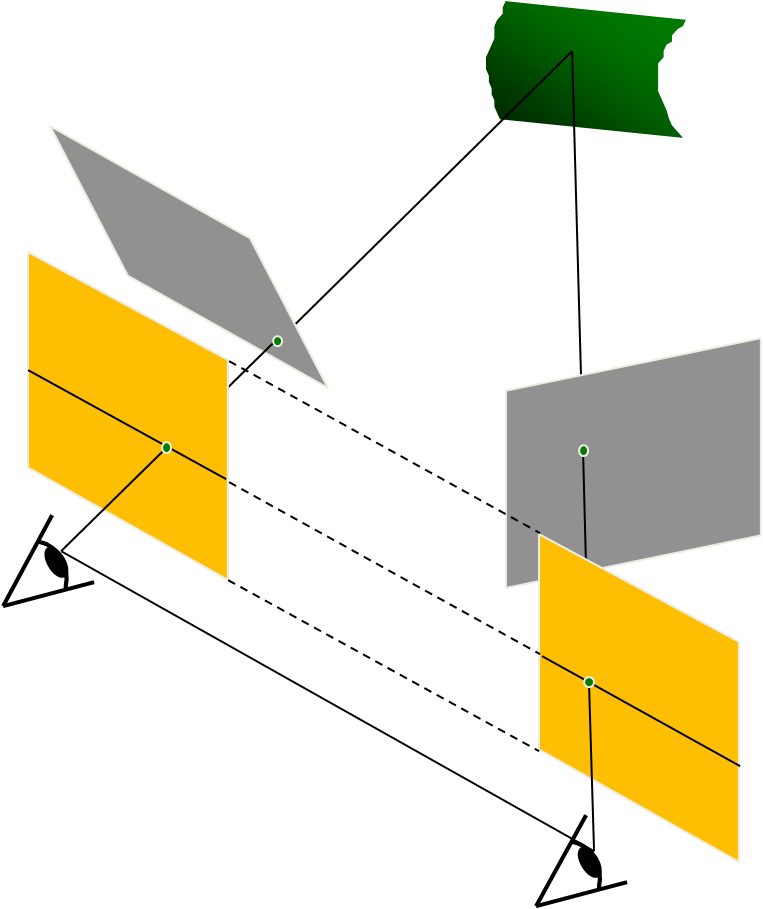
\includegraphics[width=\textwidth]{../../VIP1516/lectures/FIGURE/stereorect}
%     \column{0.4\textwidth}
%     \begin{itemize}
%     \item Reproject onto a common plane parallel to line between camera centers
%     \item Projections are homographies!
%     \item Pixel motion is horizontal after reprojection.
%     \item Cf Loop-Zhang, CVPR 1999 (Rectification is not easy)
%     \end{itemize}
%   \end{columns}
% \end{frame}


%----------------------------------------------
% \begin{frame}
%   \frametitle{Projective Rectification example}
%   \begin{center}
%     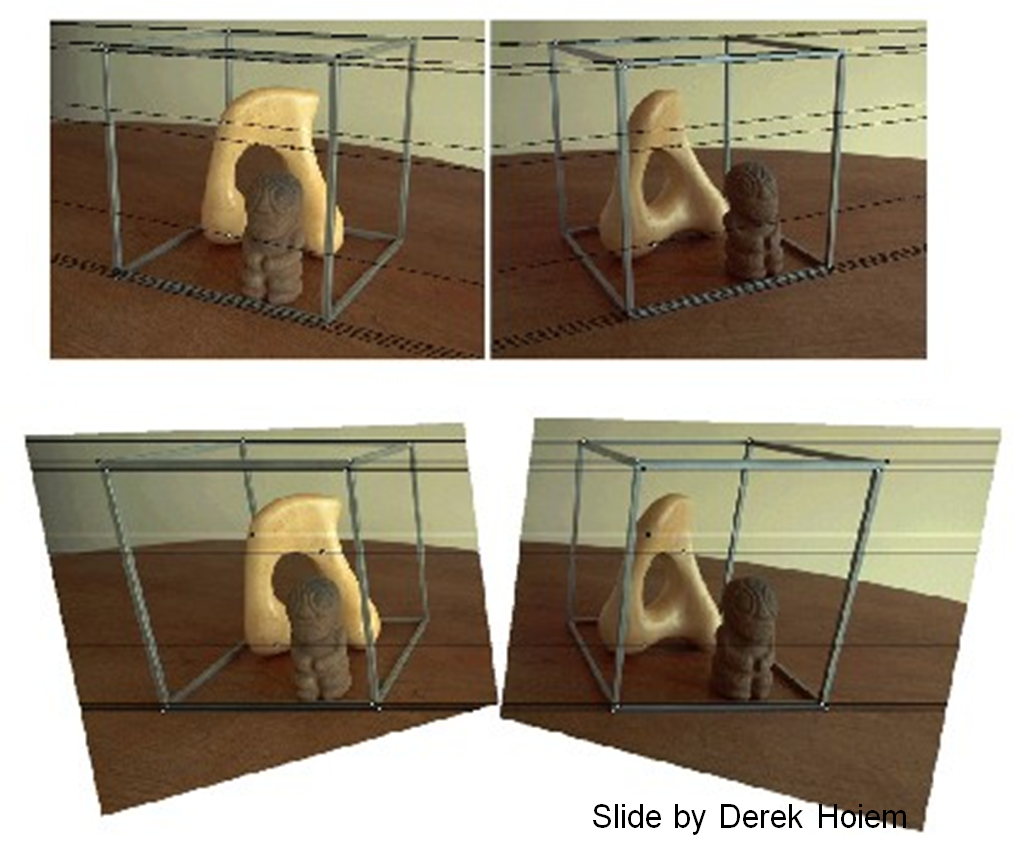
\includegraphics[width=0.8\textwidth]{../../VIP1516/lectures/IMAGES/projrectexpl}
%   \end{center}
% \end{frame}



%----------------------------------------------
\begin{frame}
\frametitle{Correspondence analysis}
Problem statement:  
{\color{blue}{Establish pairs $({\bf p_L}, {\bf p_R})$ of image 
points ${\bf p_L}$ in the left image and ${\bf p_R}$ in the
right image such that both points are projections of the same physical
scene point}}. \\[5mm]

  \begin{itemize}
  \item Correspondence analysis is the difficult part of stereo
    analysis \\[4mm]
  \item Correspondence analysis is the basic of many other
    applications, eg. stitching, geo-referencing, image
    alignment/warping etc. \\[4mm] 
  \item Most mammalians have stereo vision \\[4mm]
  \item Except for auto-focus cameras, stereo is the most widely
    applied passive  technique for 3D-measurement.
  \end{itemize}
\end{frame}





%----------------------------------------------
\begin{frame}
  \frametitle{Problems}

  \begin{minipage}{0.4\textwidth}
  \begin{itemize}
  \item Intensity in corresponding points are not equal: $E_L \neq E_R$.
  \item Many geometric properties, eg. orientation, are not preserved
    under perspective projections. 
  \item Occlusions: Things/areas visible en one image is invisible in
    the other.
  \item Double nail illusion
  \end{itemize}
  \end{minipage}
  \begin{minipage}{0.5\textwidth}
  % Show image pair with large occlusions
  % \begin{center}
  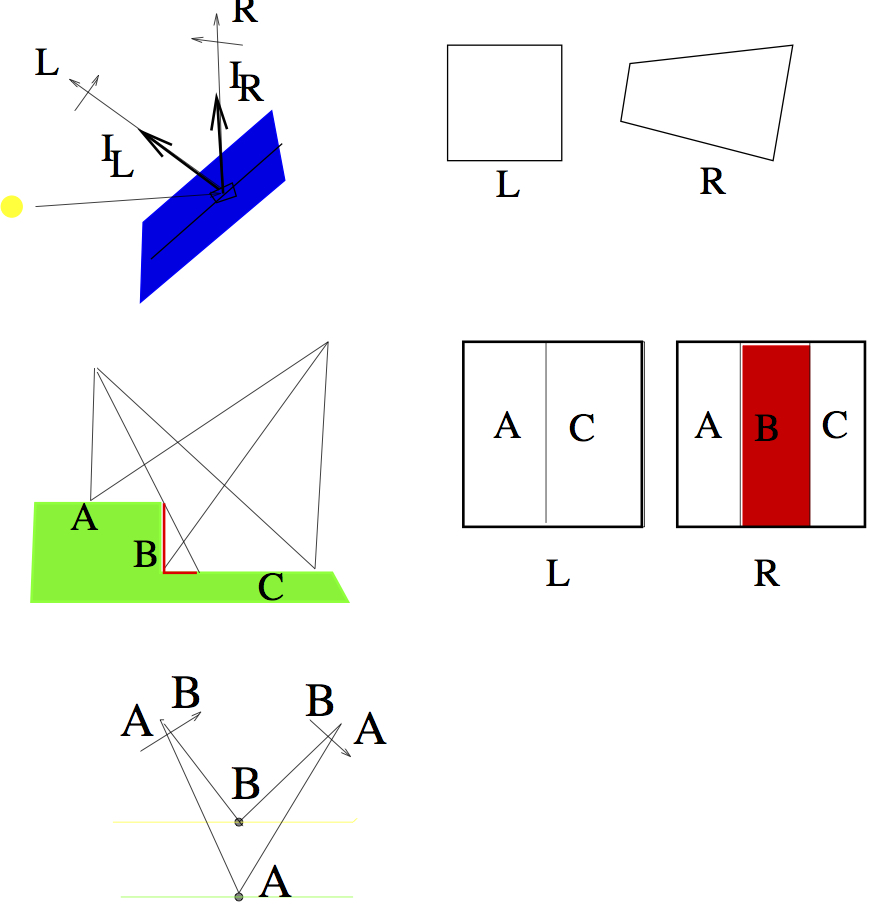
\includegraphics[width=\textwidth]{../../VIP1516/lectures/FIGURE/probilust1.jpg}
  % \end{center}
  \end{minipage}

\end{frame}





%----------------------------------------------
\begin{frame}
  \frametitle{More problems}
 \begin{itemize}
  \item Lack of texture/structure/intensity variation makes 
    makes feature matching difficult and intensity comparison
    vulnerable. 
  \item Complexity of correspondence problem: Given point in one
    image, how many possible matches exist in the other image ?
  \end{itemize}

  \begin{center}
  \includegraphics[width=0.8\textwidth]{../../VIP1516/lectures/FIGURE/kompleksitet.jpg}
  \end{center}

\end{frame}





%----------------------------------------------
% \begin{frame}
% \frametitle{Complexity}
% Assume $n$ points along both epipolar lines. $N(n)$ is number
% of solutions.
%   \begin{center}
%     \includegraphics[width=0.4\textwidth]{../../VIP1516/lectures/IMAGES/kompleksitet.jpg}
%   \end{center}
%  
% Without assumptions:  
% $N(n) \;=\; 2^{n^2}$. 
% $N(4) \;=\; 65536$ \\[2mm]
%
% Assume that each point may match at most one other point:
% $N(n) \;= \; \sum_{i = 0}^{n} \frac{(n!)^2}{(n-i)! (i!)^2}$. 
% $N(4) \;=\; 204$. \\[2mm]
%
% Assume ordering, ie. 
% $x_L^1 \leq x_L^2 \; \Rightarrow \; x_R^1 \leq x_R^2$, and uniqueness:  \\
% $N(n) \;=\; \frac{(2n)!}{(n!)^2}$. 
% $N(4) = 70$. \\[2mm]
% 
%% Assume strong ordering: All L-points match exactly one R-point: \\
% Assume all L-points match exactly one R-point: \\
% $N(n) \;=\; n!$. 
% $N(4) \;=\; 12$. \\[2mm]
% 
% Assume strong ordering and uniqueness: \\
% $N(n) \;=\; 1$.
% \end{frame}



%----------------------------------------------
\begin{frame}
  \frametitle{Simplifying assumptions}
  \begin{itemize}
  \item Intensities are similar, eg. $|E_L - E_R| \leq \theta$ or are
    spatially correlated (more later). \\[3mm]
  \item Fundamental matrix is estimated $\implies$ matching is reduced
    to 1D along epipolar lines. \\[3mm]
  \item The world consist of solid textured surfaces. Thus, the
    disparity is a single-valued function, and there exist a {\em
      unique} solution to the correspondence problem. \\[3mm]
  \item Occlusions and depth discontinuities do not exist. \\[3mm]
  \item Ordering: Corresponding points appear in the same order along
    the epipolar lines. \\[3mm]
  \item The magnitude of the disparity gradient is limited (for humans
    to about 1).    
  \end{itemize}
\end{frame}





%----------------------------------------------
% \begin{frame}
% \frametitle{Example: Large disparity gradient 1}
% 
%%  Large disparity gradient (0.6):
% \begin{center}
%   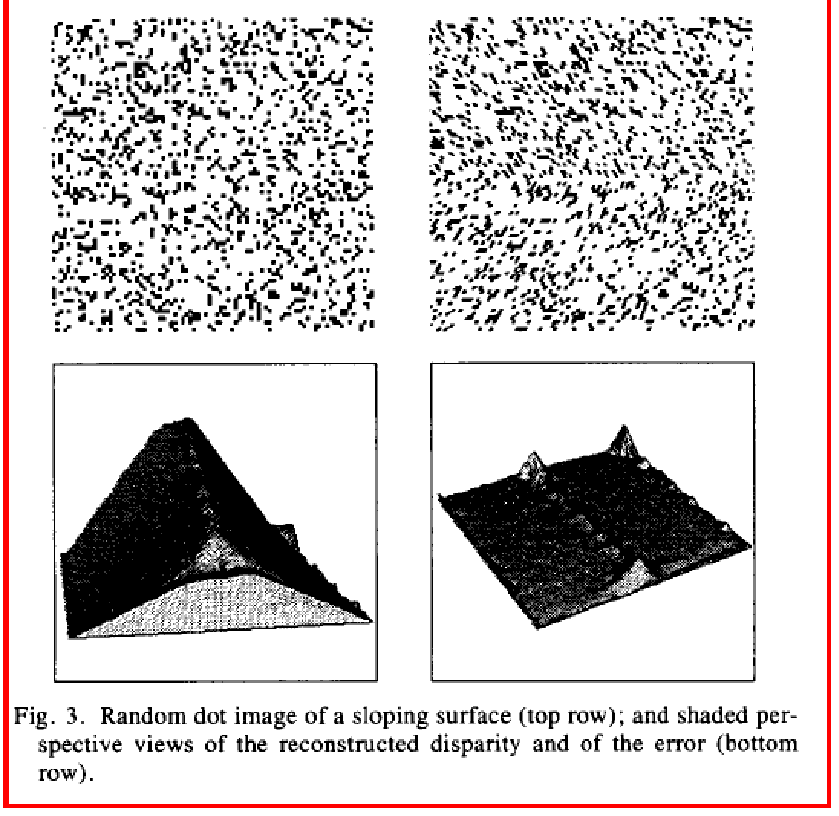
\includegraphics[width=0.6\textwidth]{../../VIP1516/lectures/IMAGES/largegradient.pdf}
% \end{center}
% 
% Humans can fuse random dot stereograms with no structural information.
% Image has a disparity gradient of 0.6. Humans cannot fuse images with
% gradient larger than 1.
% \end{frame}


%----------------------------------------------
% \begin{frame}
% \frametitle{Example: Large disparity gradient 2}
%
% \begin{center}
%   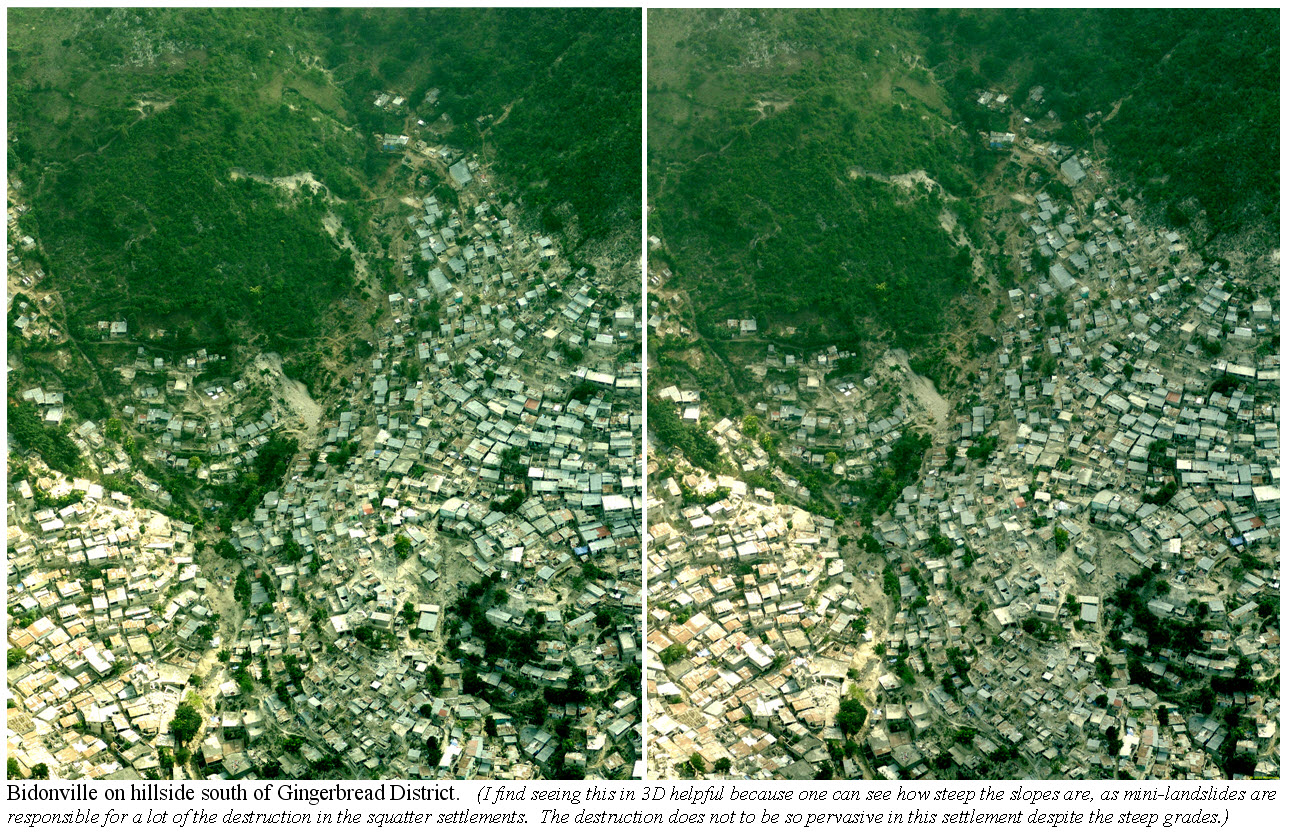
\includegraphics[width=0.9\textwidth]{../../VIP1516/lectures/IMAGES/StereoPair-of-Bidonville.jpg}
%   \end{center}
% \end{frame}





%----------------------------------------------
% \begin{frame}
% \frametitle{Example: What surface ?}
%
%% stereo image of tree - do we have surfaces ?
%   \begin{center}
%   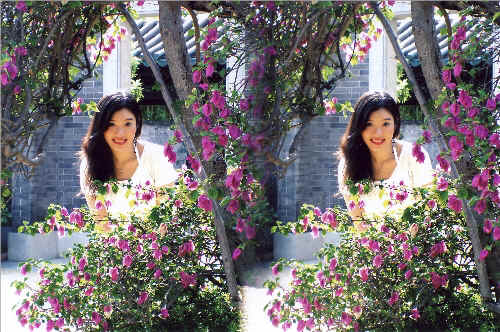
\includegraphics[width=0.9\textwidth]{../../VIP1516/lectures/IMAGES/loreo01.jpg}
%   \end{center}
% \end{frame}





% \section{Feature based vesus dense solutions}



%----------------------------------------------
\begin{frame}
  \frametitle{Correspondence analysis}
  \begin{itemize}
  \item {\color{red}{Dense intensity based methods}} may be accurate but is very
    noise sensitive and have a small capture area. Also, they may be
    computationally expensive. \\[5mm]
   \item {\color{red}{Sparse feature based methods}} is faster, more reliable, and
     have larger capture area, but results in scattered depth information.\\[3mm]
  \item {\color{blue}{Very local}} features as edge points often has a
    short descriptor, e.g. edge orientation. \\[5mm] 
  \item {\color{blue}{Less local}} features (as SIFT) is less dense, but often has a
            more expressive descriptor. \\[5mm]
  \item {\color{blue}{Large features}} (as image segments) are few and
    more easy to match, but gives less depth information. 
  \end{itemize}
\end{frame}



%----------------------------------------------
%\begin{frame}
%   \frametitle{Area based stereo}
%   \begin{itemize}
%   \item Pixelwise intensity comparison does not work. Areas, say 
%     $7 \times 7$, or $13 \times 13$ are used. Larger windows implies
%     better robustness, less precision and larger vulnerability to occlusions.
%   \item All R-windows centered and displaced along the epipolar line
%     are compared to the L-window centered at the point in question and
%     the best is chosen.
%   \item Typical measure: {\color{green}{Normalised cross-correlation}}
%   \end{itemize}
% 
% \begin{center}
%   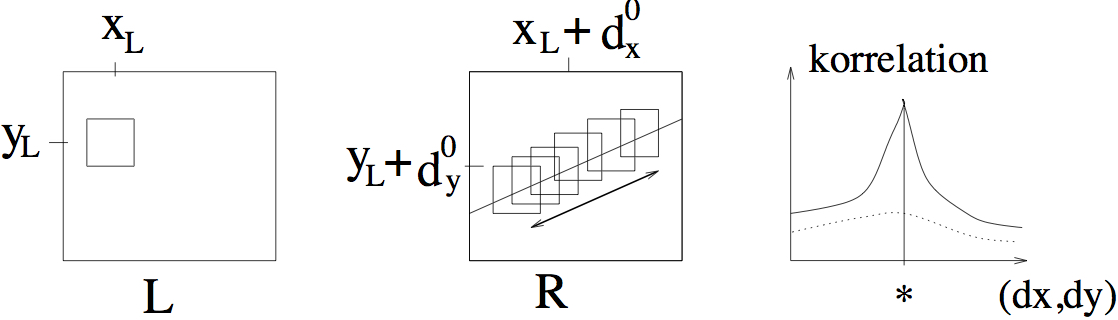
\includegraphics[width=0.9\textwidth]{../../VIP1516/lectures/FIGURE/arealstereo.jpg}
% \end{center}
% \end{frame}


%----------------------------------------------
% \begin{frame}
%   \frametitle{Disparity Map By Dense Block Matching\footnote{Slide adapted from  Derek Hoiem}}
%   \begin{center}
%     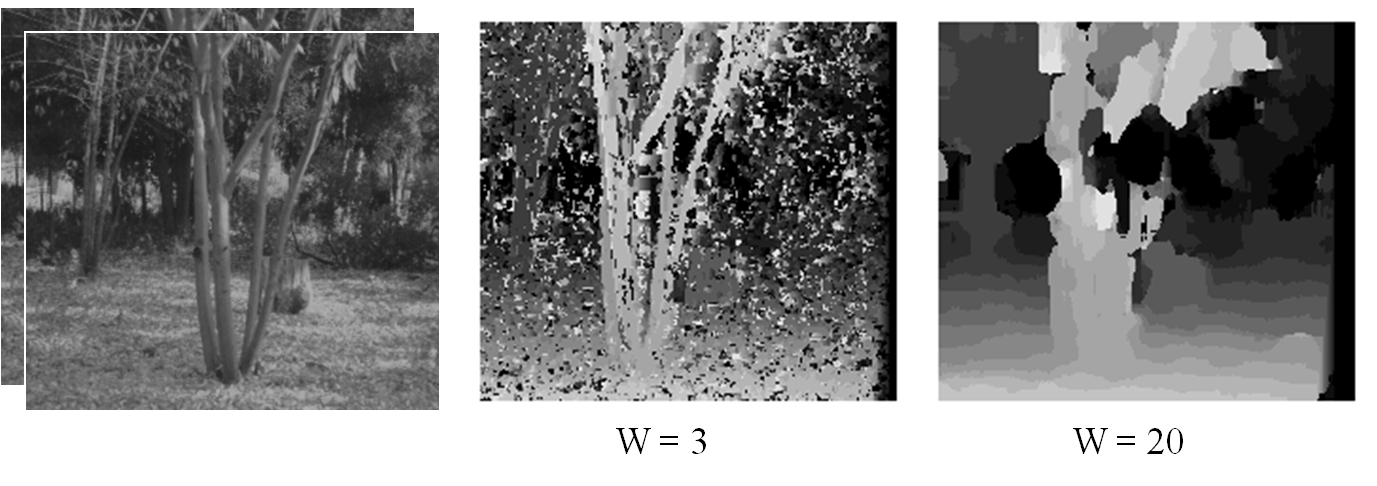
\includegraphics[width=\textwidth]{../../VIP1516/lectures/IMAGES/ddmapsblockmatch}
%   \end{center}
%   \begin{itemize}
%   \item Window size 3: Noisy but detailed.
%   \item Window size 20: smoother, but missing details.
%   \end{itemize}
% \end{frame}



%----------------------------------------------
% \begin{frame}
% \frametitle{Cross-correlation}
% The cross-correlation between two continuous functions (with limited
% square integral) is defined by:
% \begin{displaymath}
%   h(x) = (f \circ g)(x) \;\;=\;\; \int
%         f^{\star}(\alpha) g(x \;+\; \alpha) d\alpha
% \end{displaymath}
% 
% Discrete normalised 2D cross correlation is defined by:
% \begin{displaymath}
% \frac{1}{n} \sum_{(x,y) \in \Omega} 
%     \frac{(f(x,y) - \bar{f}) \cdot  (g(x + \alpha,y + \beta) - \bar{g})}
%     {\sigma_f \sigma_g}
% \end{displaymath}
% where $n$ is the number of pixels in $\Omega$, $\bar{f}$ is the mean
% value of $f$ in $\Omega$, $\sigma_f$ is the standard deviation of $f$
% within $\Omega$ (and similarly for $g$).
% \medskip
%
% Cross-correlation is used in {\color{red}{Template matching}}
% where we are searching for positions in $f(x,y)$ where the
% signal/image is identical/similar to the prototype $g(x,y)$.  
% Such positions can be identified as the local maxima's of 
% $(f \circ g)(x,y)$.
% \end{frame}




%----------------------------------------------
% \begin{frame}
% Cross-correlation between an image and a prototype and the image 
% patches centered at the local maximum.  \\
%
% \begin{tabular}{l c r}
%   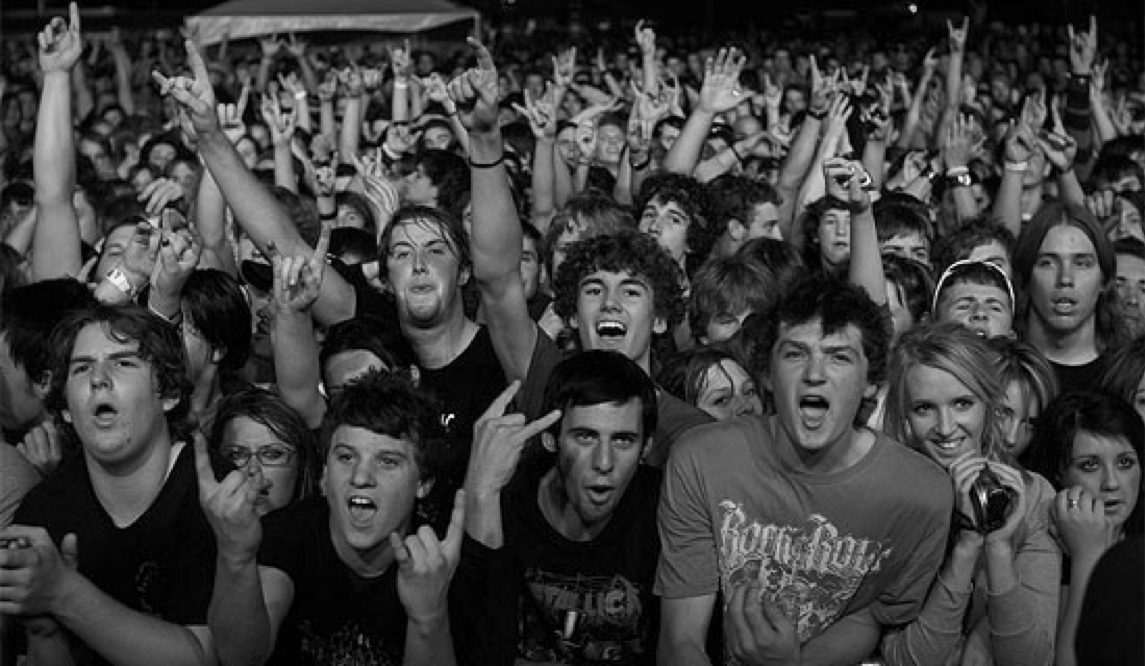
\includegraphics[width=4.8cm]{../../VIP1516/lectures/FIGURE/crowd.eps} 
%   & \hspace{2mm} & 
%%  \begin{center}
%       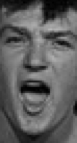
\includegraphics[width=0.35cm]{../../VIP1516/lectures/FIGURE/face.eps} \hspace{2.0cm}
%%  \end{center}
%   \\
%   \includegraphics[width=4.8cm]{../../VIP1516/lectures/FIGURE/correlres.eps} 
%   & \hspace{2mm} & 
%   \includegraphics[width=4.8cm]{../../VIP1516/lectures/FIGURE/corrresult.eps} 
% \end{tabular}
%
% \end{frame}





%----------------------------------------------
% \begin{frame}
%   \frametitle{Feature base stereo}
%   \begin{itemize}
%   \item Which feature ? \\[3mm]
%   \item For depth reconstructions, the density of points should be
%     maximised. Often edge points localised with sub-pixel accuracy is
%     chosen. \\[3mm]
%   \item For matching efficiency, the quality (disambiguation power) of
%     the descriptor should be maximised.  This is computational more
%     expensive. Often corners or blobs with SIFT/HOG-like descriptors
%     are used. \\[3mm]
%   \end{itemize}
%
% In practice hybrid systems may be used:  Sparse descriptive feature
% points are used for fundamental matrix estimation.  Edge points are
% used to obtain an initial reconstruction. Finally, intensity based
% methods are used for fine-tuning and filling-in.
% \end{frame}



% \section{Scale-space and Coarse-to-fine}



%----------------------------------------------
% \begin{frame}
%  \frametitle{3-Camera stereo}
%
% The use of 3 cameras in stereo vision, and assuming all fundamental
% matrices known, makes the correspondence analysis more easy and
% robust. 
%
% \begin{center}
%       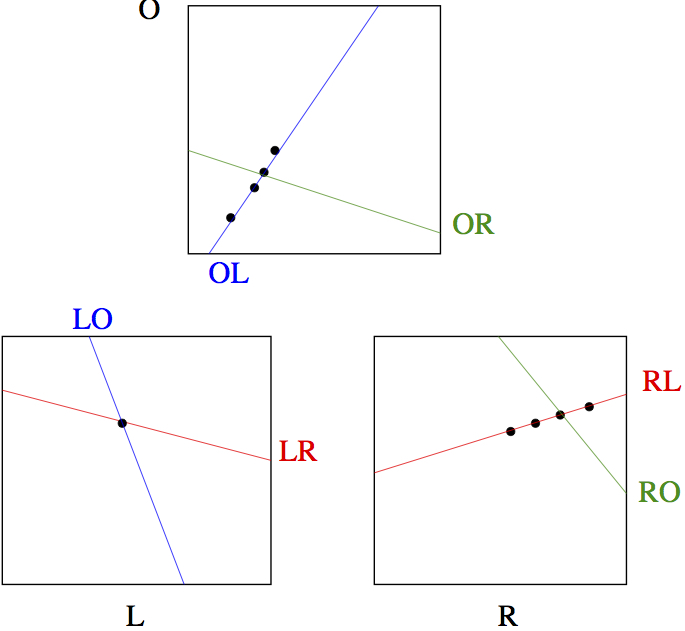
\includegraphics[width=0.6\textwidth]{../../VIP1516/lectures/FIGURE/kamera3.jpg}
% \end{center}
%
% \end{frame}



%----------------------------------------------
% \begin{frame}
% \frametitle{Scale-Space -repetition}
% Often we don't know the size of the things we are imaging, so we have
% to use both large and small filters when we analyse images. In
% practice we represent each image at a number of scales. \\[6mm]
%
% A scale-space representation is obtained by convolving the image with
% Gaussian kernels of increasingly larger size.
%
% % Please check previous slides for the definition and details on
% % scale-space. \\[6mm] 
% At small scales we only blur the images slightly to attenuate noise.
% At large scale we blur heavily to ensure that only large scale
% structures survive. \\[6mm]
% 
% % The 2D-Gaussian filter has a number of unique properties, that makes
% % it the default smoothing filter.  \\[3mm]
%
% To save space and (in particular) time we subsample the smoothed image
% versions. The result is an image pyramid.
%
% % Often the large scale images are subsampled (according to the sampling
% % theorem) to save space and to improve processing time.  
% \end{frame}




%----------------------------------------------
% \begin{frame}
% \frametitle{Pyramid representations}
% A typical pyramid representation may involve 3-10 pyramid
% levels obtained by successive Gaussian low-pas-filtering and 
% sub-sampling with a reduction factor of 2.
% 
% \begin{center}
%   \includegraphics[width=6cm]{../../VIP1516/lectures/FIGURE/pyramide.eps}
% \end{center}
%
% \end{frame}






%----------------------------------------------
% \begin{frame}
% \frametitle{How to do it in MATLAB}
% 
% A banale implementation with known number of pyramid levels: \\[3mm]
% 
% {\texttt
% \noindent
% I0 = imread(inputimage); \\
% I1 = impyramid(I0, 'reduce'); \\
% I2 = impyramid(I1, 'reduce'); \\
% I3 = impyramid(I2, 'reduce'); \\
% }
% \bigskip
%
% The code below does not work in MATLAB because Pyr is a cube and not a  
% pyramid: \\[3mm]
% 
% {\texttt
% \noindent
% gaussfilt = fspecial('gaussian', 5, 1.4); \\
% Pyr          = zeros(dimx, dimy, Nscales); \\
% Pyr(:,:,1)  = Image; \\
% for scale = 2:Nscales \\
% \hspace{1cm}  smo  = 
%      imfilter(Pyr(:,:,scale-1), gaussfilt, 'replicate', 'same'); \\
% \hspace{1cm}  Pyr(:,:,scale) = smo(1:2:end,1:2:end); \\
% end 
% }
% \end{frame}





%-------------------------------------------------------------------
% \begin{frame}
% \frametitle{The isotropic Gaussian filter} 
% \begin{displaymath}
%   G_{\sigma}(x,y) = \frac{1}{2\pi \sigma^2} 
%                    e^{- \frac{x^2 + y^2}{2 \sigma^2}}
% \end{displaymath}
% have a large number of unique features (in addition to being
% linear, position invariant, isotropic, separable) including:
% \begin{itemize}
%  \item $G_{\sigma_1} \star G_{\sigma_2} = 
%        G_{\sqrt{\sigma_1^2 + \sigma_2^2}}$ 
%  \item $G_{\sigma} \bowtie G_{\frac{1}{2 \pi\sigma}}$ 
%  \item $\lim_n F \star^n F \; = \; G_{\sigma}$
%  \item $G_{\sigma}$ is simultaneously optimally concentrated
%        in the spatial as well as the frequency domain.
%  \item $G_{\sigma}$ is the solution to the heat equation 
% %       (see proof in J\"{a}hne section 5.3.1):
%        $f_{t} = k \cdot [ f_{xx} + f_{yy} ]$, with time defined by
%        $t = \frac{\sigma^2}{2}$.
%  \item $G_{\sigma}$ is the only filter satisfying both the
%        {\em semi-group property} and the 
%        {\em minimum-maximums principle} 
%%     (see J\"{a}hne section 5.3.2).
%        Both features are essential for a multi-scale representation.
% \end{itemize}
% \end{frame}


%-------------------------------------------------------------------
% \begin{frame}
% \frametitle{Scale-space time series of a signal}
%
% \begin{center}
%   \includegraphics[width=9.0cm,height=7.0cm]{../../VIP1516/lectures/FIGURE/scspfig.eps}% 
% \end{center}
%
% Each signal is lifted with a value about 20 above the previous 
% scale-space slice to make the evolution of the signal more visible.
% \end{frame}





%----------------------------------------------
% \begin{frame}
% \frametitle{Coarse-to-fine}
% Pyramid-based coarse to fine approaches:
%
% \begin{itemize}
%   \item reduce the time complexity from $\mathcal{O}(N)$ to
%     $\mathcal{O}(\log(N))$.  \\[3mm]
%   \item reduce the complexity of the correspondence problem with a
%     large factor (see previous slide). \\[3mm]
%   \item Facilitates global operations using only local computations \\[3mm]
% \end{itemize}
% \bigskip
%
% Principle: Use approximate solutions obtained at higher pyramid level
% to constrain the search at lower levels.
% \end{frame}


%----------------------------------------------
% \begin{frame}
% \frametitle{Coarse-to-fine Stereo}
%
% \begin{minipage}{0.30\textwidth}
% In practice the disparity may be large (several hundred pixels) and
% have large variation (eg. from -50 to +50 pixels).  To reduce the size
% of the search area we need an estimate of the disparity. 
% \end{minipage}
% \begin{minipage}{0.69\textwidth}
% \begin{center}
%   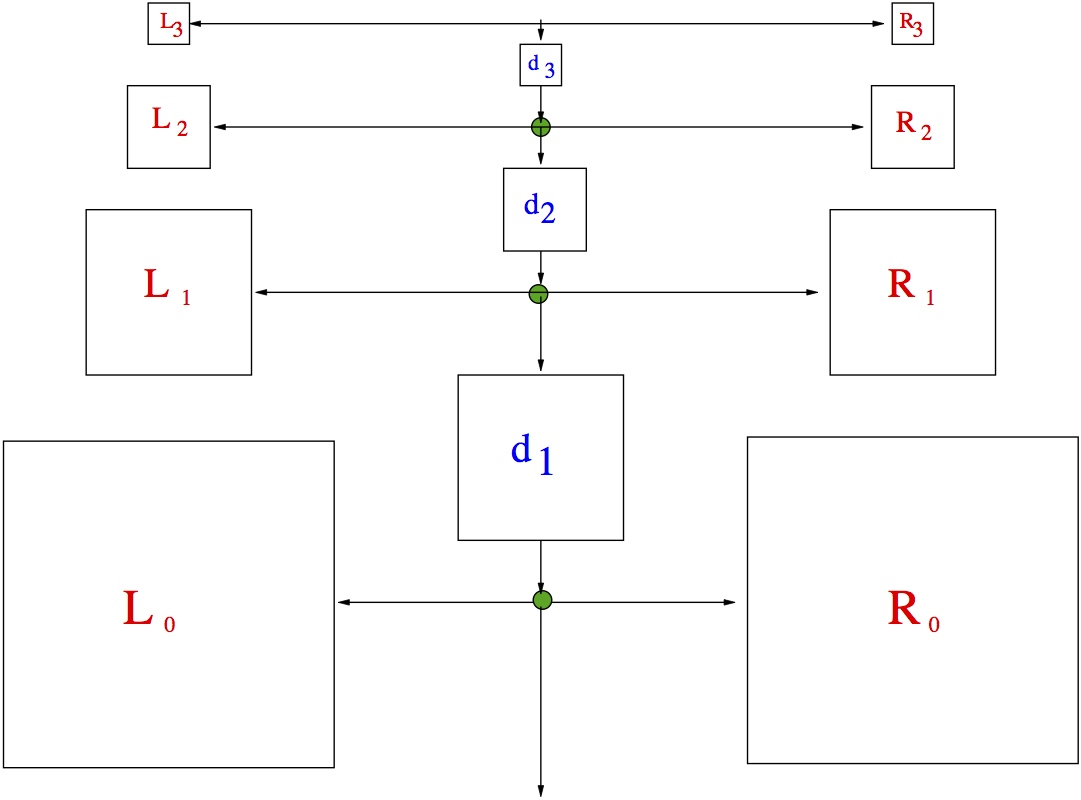
\includegraphics[width=0.75\textwidth]{../../VIP1516/lectures/FIGURE/grovfin.jpg} 
% \end{center}
% \end{minipage}
%
% {\footnotesize
% \begin{center}
% {\color{darkgreen}{Method: Succesive smoothing and downsampling}} 
% \end{center}
% The total space requirement is: 
% \begin{displaymath}
%   1 \;+\; \frac{1}{4} \;+\; \frac{1}{16} \;+\; \cdots \;<\; \frac{4}{3}
% \end{displaymath}
% }
% \end{frame}



%----------------------------------------------
% \begin{frame}
%  \frametitle{Example}
% \begin{center}
%   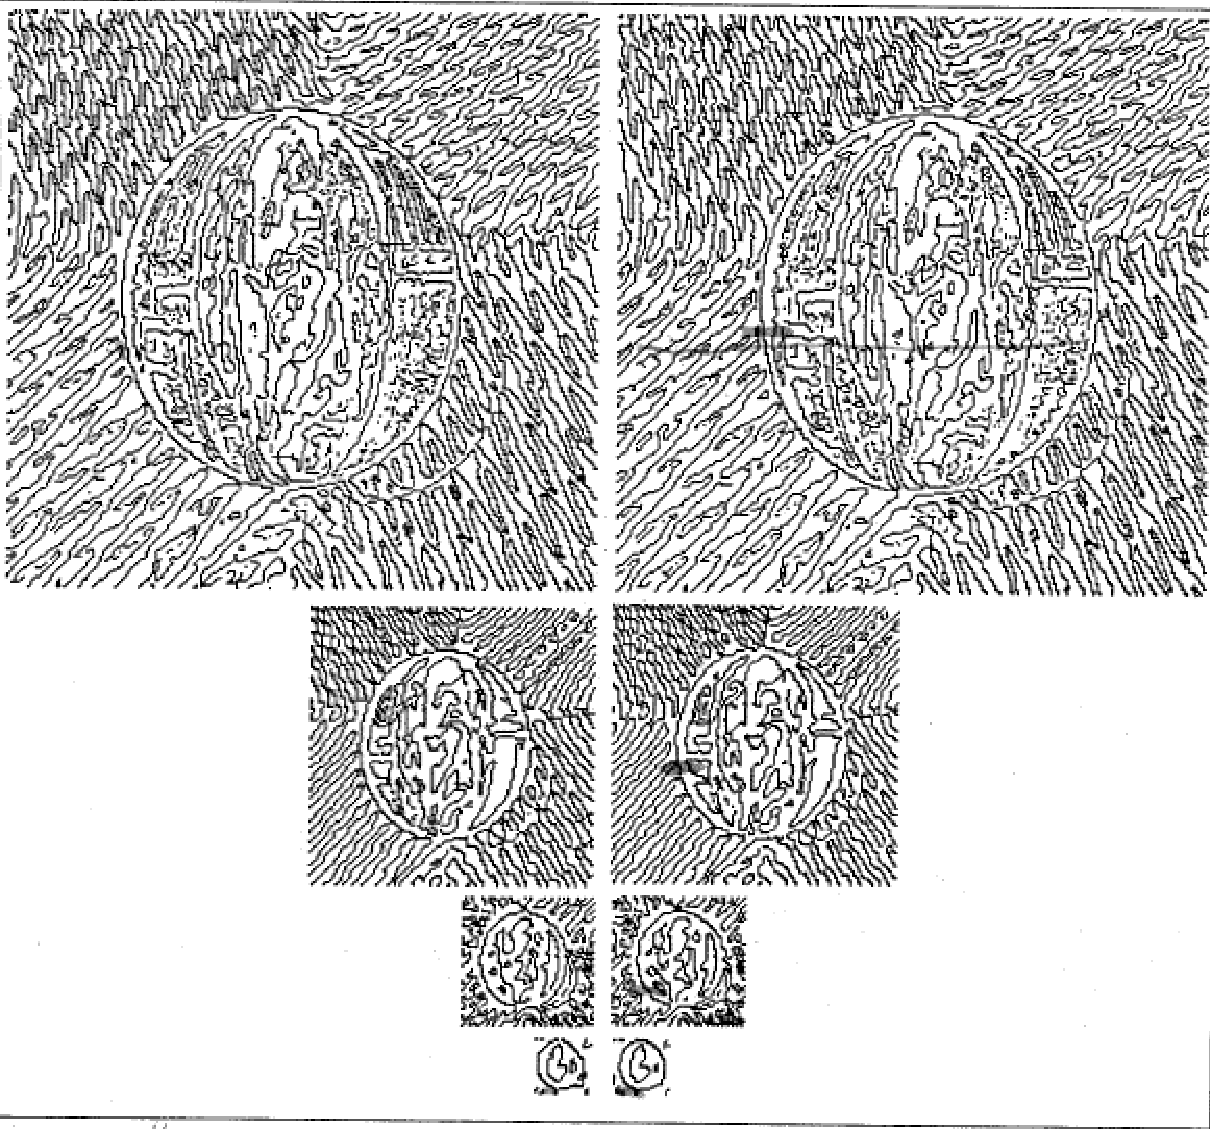
\includegraphics[width=0.8\textwidth]{../../VIP1516/lectures/MyImages/EdgePyramidStereo2.pdf} 
% \end{center}
% \end{frame}




%----------------------------------------------
% \begin{frame}
%   \frametitle{Surface interpolation}
%%   \begin{itemize}
%%   \item Region growing (from point values)
%%   \item Planar surface interpolation using Delaunay triangulation
%%   \item Thin plate spline approximation using iterative updating. 
%%    \end{itemize}
% 
% It is possible to fit a thin plate spline surface to the estimated
% sparse depth measurements. Usually, an (slow) iterative updating is
% used. To speed up a simple and fast method is used to obtain a initial 
% estimate. 
% \bigskip
%
% Surface interpolation is too advanced for this course.
% \end{frame}




%----------------------------------------------
% \begin{frame}
% \frametitle{Reconstruction on few data}
% The results below are produced by a MATLAB-program
% {\color{blue}{interp(.)}} used in VIP-assignment 3 (2014).
% \begin{center}
%   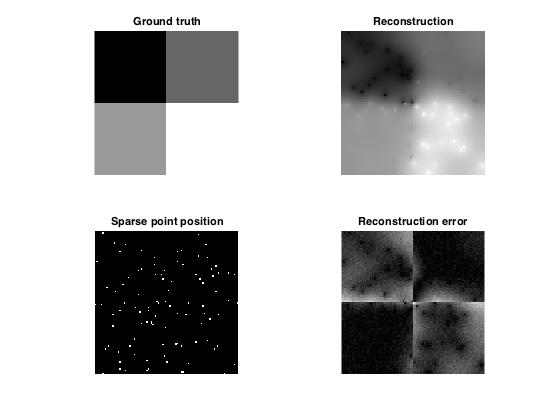
\includegraphics[width=7.0cm]{../../VIP1516/lectures/MyImages/RECfewdata.jpg} 
% \end{center}
% Very sparse data, like SIFT-points makes reconstruction hard.
% \end{frame}



%----------------------------------------------
% \begin{frame}
% \frametitle{Reconstruction on more data}
% Dense data like edge points makes reconstruction better.
% 
% \begin{center}
%   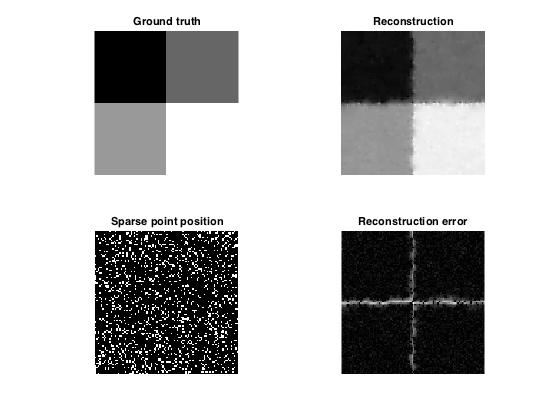
\includegraphics[width=7.0cm]{../../VIP1516/lectures/MyImages/RECmanydata.jpg} 
% \end{center}
% 
% \end{frame}



%----------------------------------------------
% \begin{frame}
%   \frametitle{Discontinuities and occlusion}
%   \begin{itemize}
%   \item It is possible to perform discontinuous regularisation, where
%     the smoothness term is disregarded when the surface is bended more
%     than some threshold. \\[3mm]
%   \item Discontinuities are accompanied by occluded areas. If any
%     point in an occluded area is matched it will be wrong. If not, the
%     surface will be reconstructed more smooth than what it should. \\[3mm]
%   \end{itemize}
%
% \begin{center}
%   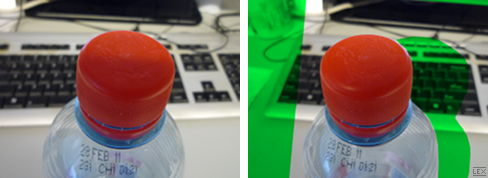
\includegraphics[width=7.0cm]{../../VIP1516/lectures/MyImages/3d-occlusion.jpg} 
% \end{center}
% \end{frame}



%----------------------------------------------
% \begin{frame}
%   \frametitle{Enforcing Smoothness}
% 
%   Mostly, the 3D world is piecewise smooth. Occasionally, thin
%   elongated structures may occur, but mostly the scene can be divided
%   into large patches of slowly varying disparity. \\[3mm]
% 
%   All stereo algorithms have to assume/enforce some kind of disparity
%   smoothness to perform well.  The quality of the result depends
%   highly on how this is done. \\[3mm]
% 
%   One simple approach is to replace any uncertain disparity estimate
%   with a local average of trusty neighboring estimates. The 
%   credibility of a candidate match may depend on the data term (cross
%   correlation value) and/or the number of competing candidates.
% \end{frame}



%----------------------------------------------
% \begin{frame}
%   \frametitle{Assignment 3}
%
%   In assignment 3 you have to develop a method for stereo
%   correspondence analysis using dense normalised cross correlation.\\[3mm]
% 
%   You will have to face problems like how to do coarse-to-fine
%   analysis, how to implement a pyramid structure, and how to enforce
%   (piecewise) smoothness.  \\[3mm]
%
%   You may choose to handle depth/disparity discontinuities and
%   occlusions, but this is not recommended (to start with).\\[3mm]
%
%   In the following you will se some results of a test solution to
%   assignment 3.
% \end{frame}



%----------------------------------------------
% \begin{frame}
%   \frametitle{Venus}
%   Result of applying a minimal solution to assignment 3, 2017/18.
%    \begin{center}
%     \includegraphics[width=0.95\textwidth]{../../VIP1718/SLIDES/Images/VenusResult.jpg}
%   \end{center}
% \end{frame}



%----------------------------------------------
% \begin{frame}
%   \frametitle{My Venus result}
%   Result of applying a minimal solution to assignment 3, 2017/18.
%    \begin{center}
%     \includegraphics[width=0.9\textwidth]{../../VIP1718/SLIDES/Images/VenusDISP.jpg}
%   \end{center}
% \end{frame}




%----------------------------------------------
% \begin{frame}
% \frametitle{Tsukuba}
% {\tiny
% The images in this and the next slides are from Scharstein, Szeliski:
% {\em A taxonomy and Evaluation of Dense Two-Frame Stereo
%   Correspondence Algorithms}, Int.Jour. of Comput.Vis. 47, 2002.
%  See: \url{http://vision.middlebury.edu/stereo/data/}.
% }
%
%  \begin{center}
%   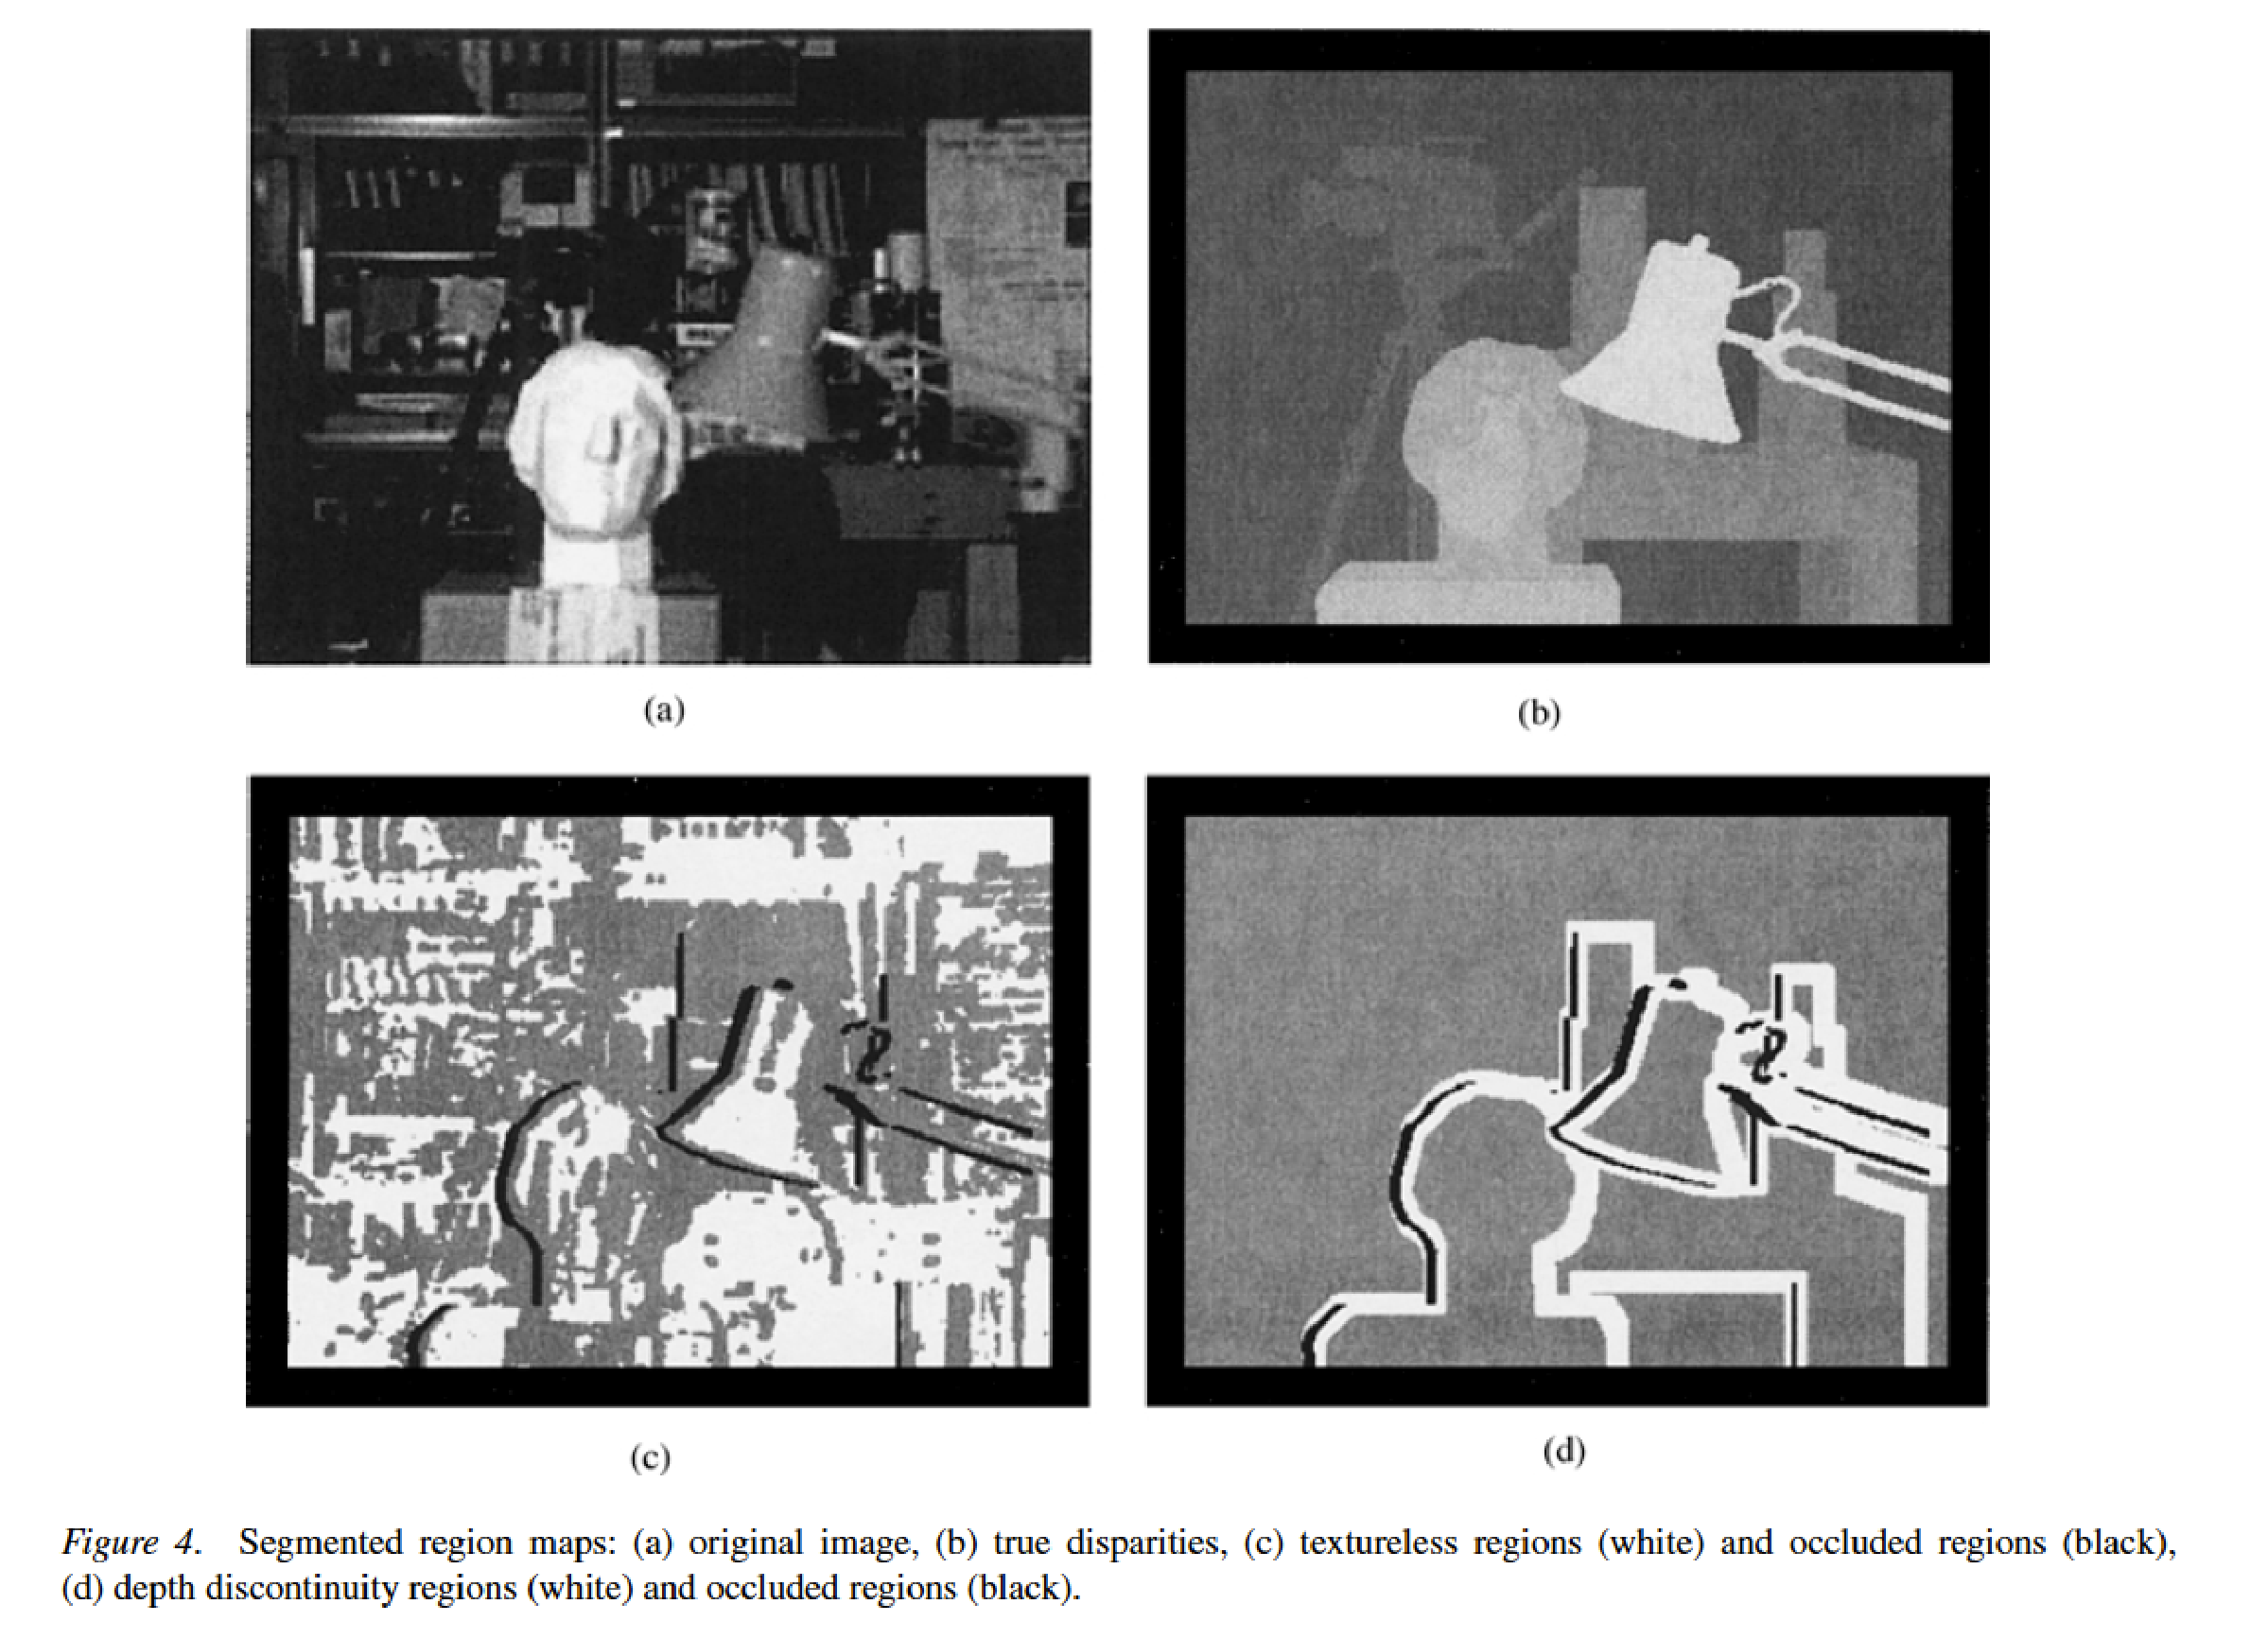
\includegraphics[width=8.0cm]{../../VIP1516/lectures/MyImages/ImStolen.pdf} 
% \end{center}
% \end{frame}



%----------------------------------------------
% \begin{frame}
% \frametitle{Other peoples results}
%  \begin{center}
%   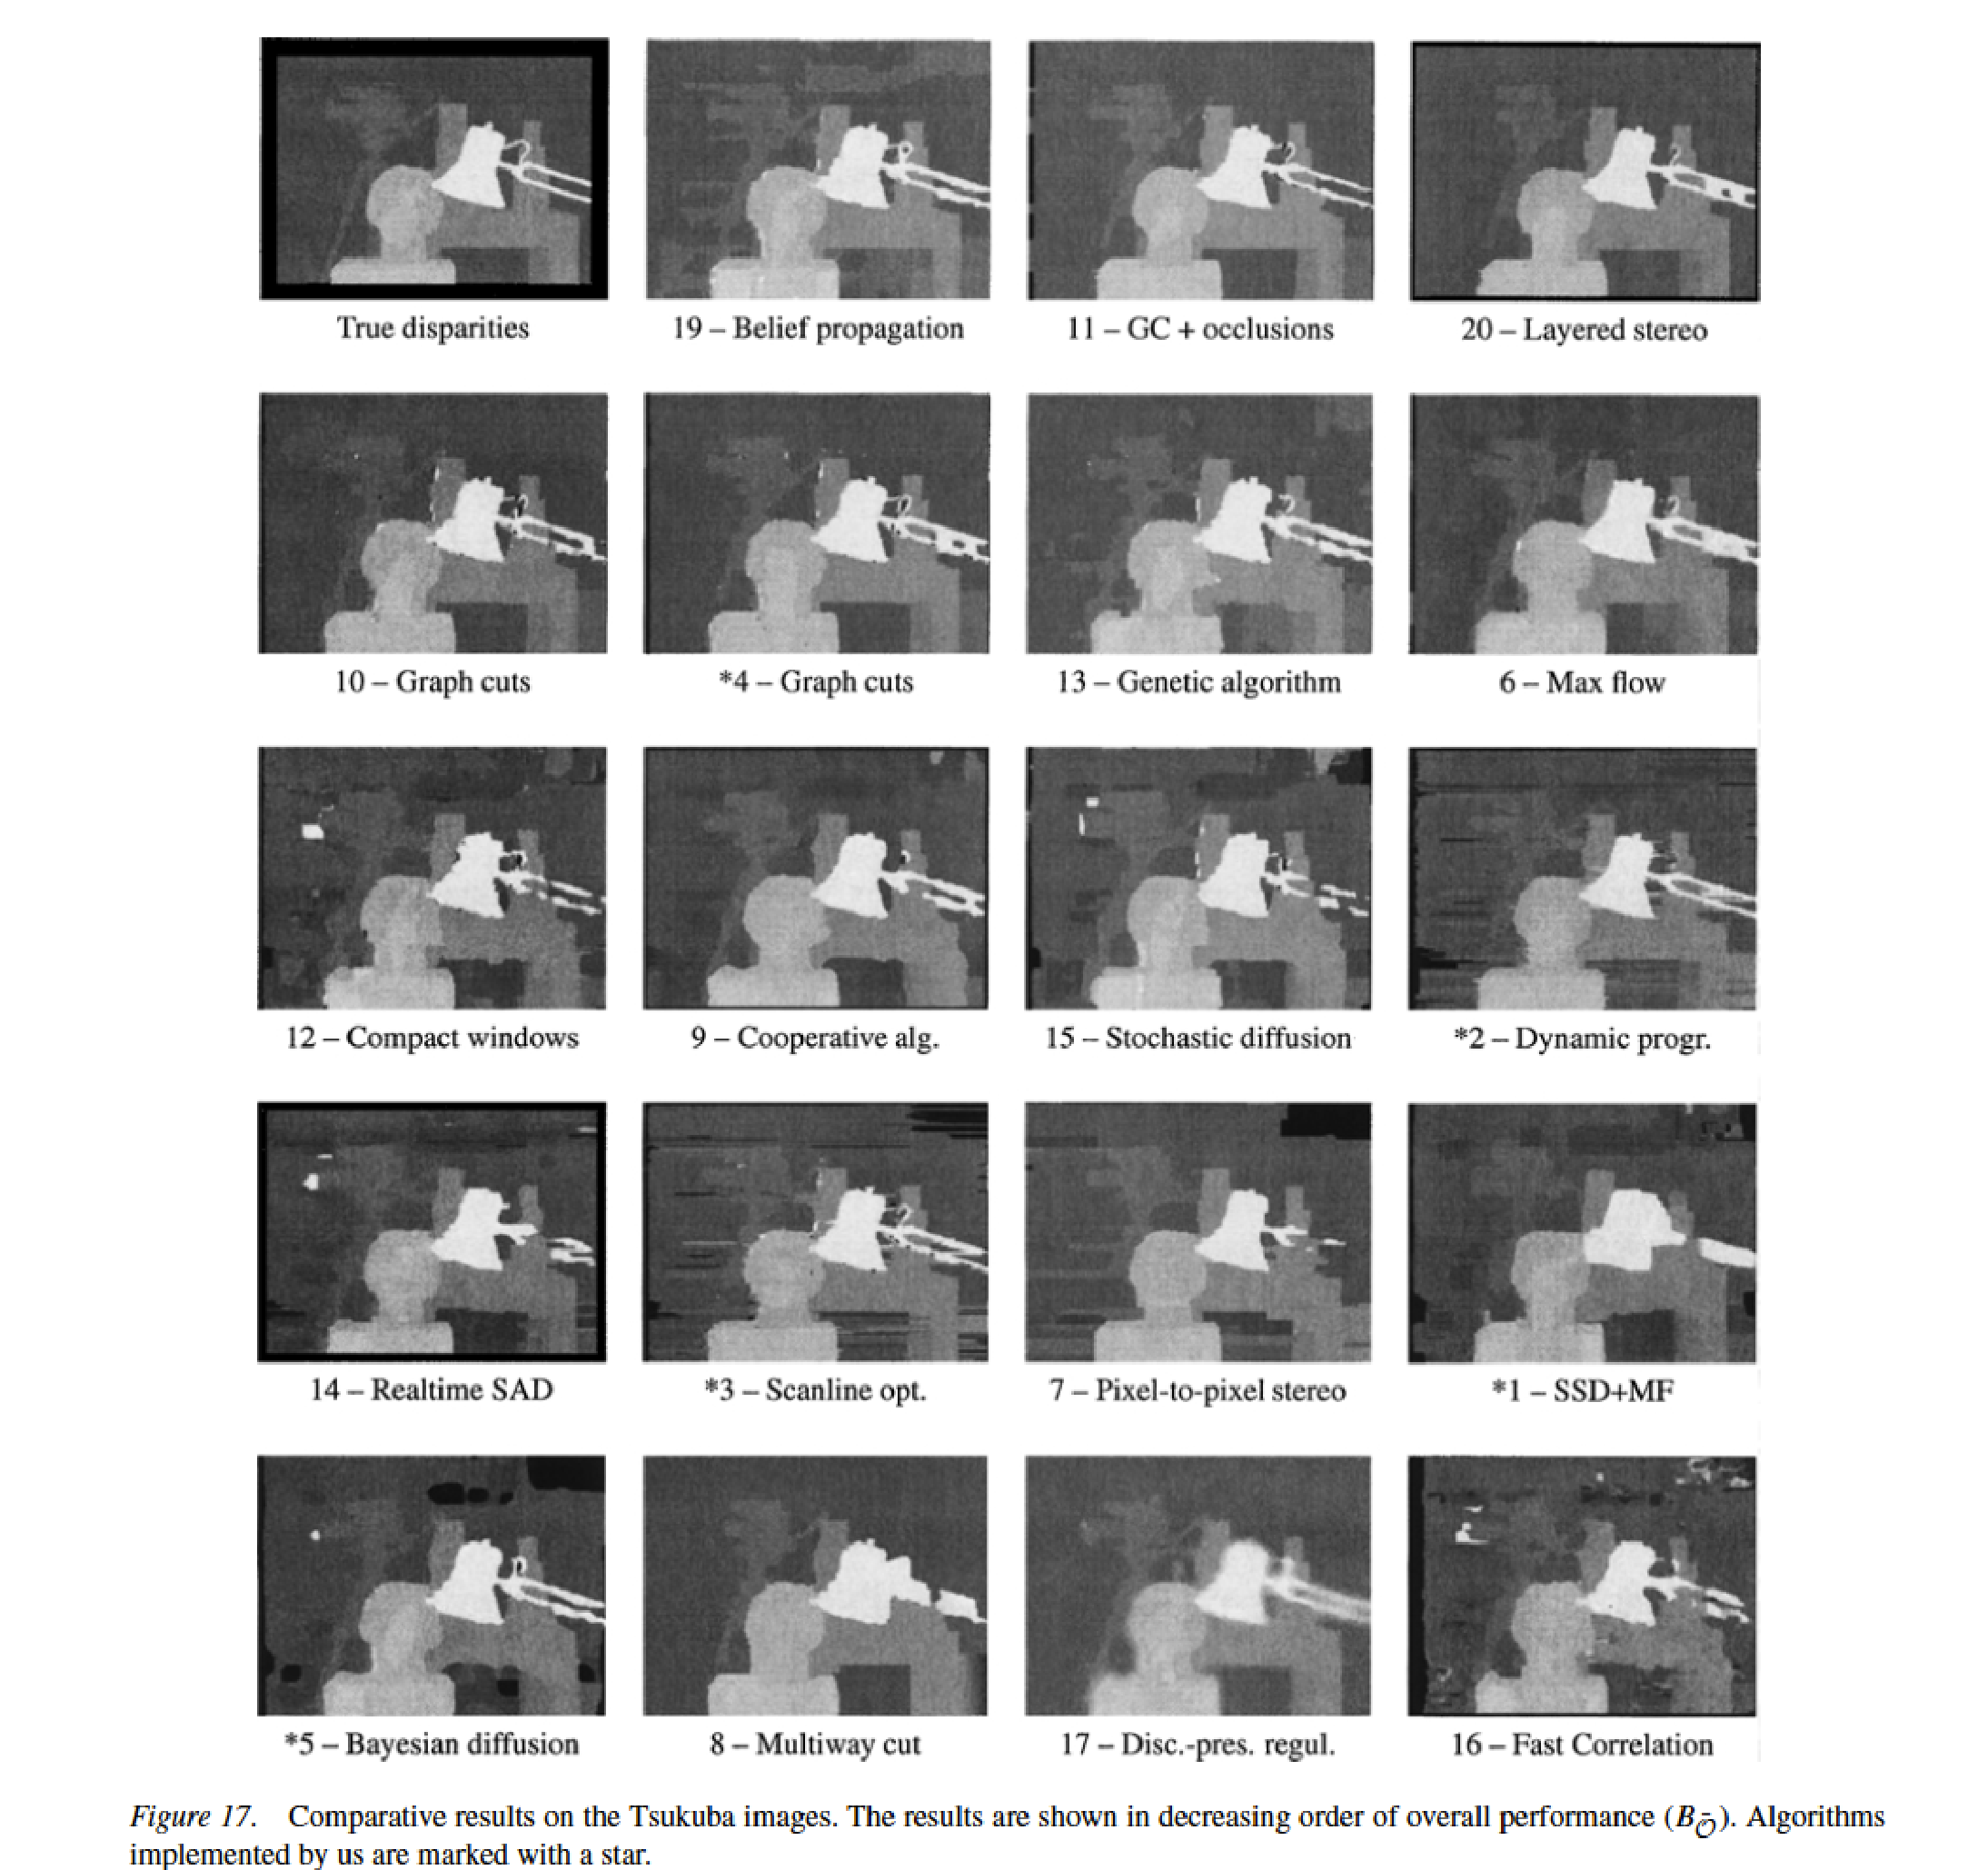
\includegraphics[width=9.0cm]{../../VIP1516/lectures/MyImages/ImStolen2.pdf} 
% \end{center}
% \end{frame}

%----------------------------------------------
% \begin{frame}
%   \frametitle{Tsukuba}
%   Result of applying a minimal solution to assignment 3, 2017/18.
%    \begin{center}
%     \includegraphics[width=0.95\textwidth]{Images/TsukubaResults.jpg}
%   \end{center}
% \end{frame}



%----------------------------------------------
% \begin{frame}
%   \frametitle{My Tsukuba result}
%   Result of applying a minimal solution to assignment 3, 2017/18.
%    \begin{center}
%     \includegraphics[width=0.9\textwidth]{Images/TsukubaDisp.jpg}
%   \end{center}
% \end{frame}


%----------------------------------------------
% \begin{frame}
%   \frametitle{Other methods}
% You may find many other approaches in the literature, eg.
% a Dynamic-programming approach, See Forsyth and Ponce 2ed. 
% Section 7.5.2.
%\bigskip
%
%  \begin{center}
%    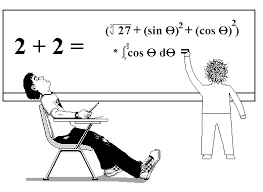
\includegraphics[width=0.5\textwidth]{../../VIP1516/lectures/MyImages/keepitsimple.png}
%  \end{center}
% 
% For assignment 3, you are advised to do something simple that
% you might get to work rather than more advanced methods.
% \end{frame}




%----------------------------------------------
% \begin{frame}
%   \begin{center}
%    \includegraphics[width=\textwidth]{../../VIP1516/lectures/IMAGES/tired}
%  \end{center}
% \end{frame}



% Below is for the exercises
%----------------------------------------------
% \begin{frame}
% \frametitle{Pentagon images}
%
%    \begin{center}
%     \includegraphics[width=0.45\textwidth]{../../VIP1516/lectures/MyImages/PentagonR.jpg}
%     \hspace{2mm}
%     \includegraphics[width=0.45\textwidth]{../../VIP1516/lectures/MyImages/PentagonL.jpg}
%   \end{center}
% \end{frame}




%----------------------------------------------
% \begin{frame}
% \frametitle{Dense correlation based matching}
% Result of applying a minimal solution to assignment 3, 2017/18.
% 
%    \begin{center}
%     \includegraphics[width=0.95\textwidth]{Images/PentagonResults.jpg}
%   \end{center}
% 
% \end{frame}


%----------------------------------------------
% \begin{frame}
% \frametitle{Dense correlation based matching}
% Result of applying a minimal solution to assignment 3, 2017/18.
% 
%    \begin{center}
%     \includegraphics[width=0.9\textwidth]{Images/PentagonDisp.jpg}
%   \end{center}
%
% \end{frame}




%----------------------------------------------
% \begin{frame}
% \frametitle{Edge based matching}
% Method uses coarse to fine matching of edge points and surface
% interpolation to achieve a dense disparity. Output of 110-lines of
% code programs to verify VIP-assignment 3 in 2014:
%    \begin{center}
%     \includegraphics[width=0.6\textwidth]{../../VIP1516/lectures/MyImages/showdispPentagon2.png}
%   \end{center}
% \end{frame}

%----------------------------------------------
% \begin{frame}
% \frametitle{Venus}
%    \begin{center}
%    \includegraphics[width=0.45\textwidth]{../../VIP1516/lectures/MyImages/VenusR.png}
%    \hspace{2mm}
%    \includegraphics[width=0.45\textwidth]{../../VIP1516/lectures/MyImages/VenusL.png}
%  \end{center}
% \end{frame}

%----------------------------------------------
% \begin{frame}
% If you get something similar your can be satisfied.
%    \begin{center}
%     \includegraphics[width=0.4\textwidth]{../../VIP1516/lectures/MyImages/GtVenus.jpg}
%     \hspace{2mm}
%    \includegraphics[width=0.5\textwidth]{../../VIP1516/lectures/MyImages/showdispVenus.jpg}
%  \end{center}
% \end{frame}





% ============================================
%  Stitching (new)
%----------------------------------------------
% \begin{frame}
% \frametitle{Stitching}
% In stitching, or panorama making, several images are combined into one
% larger image. 
%
% \begin{center}
%     \includegraphics[width=0.64\textwidth]{../../../ATIA/lectures/IMAGES/stitching.jpg}
% \end{center}
%
% A standard transformation technique is to map the images through
% homographies. However, this requires that the transformed scene
% surface is planar.  Obviously this often is not the case. 
% 
% \end{frame}


%----------------------------------------------
% \begin{frame}
% \frametitle{Stitching techniques}
% Another approach is to divide the resulting image in patches and apply
% homographies to each. This obviously requires a constraint that
% transformations from neighboring patches agree. This ends up in a
% global optimization for the local homographies, but under
% regularization of a set of compatibility constraints.
%
% \begin{center}
%    \includegraphics[width=0.80\textwidth]{../../../ATIA/lectures/IMAGES/StitchingPatches.pdf}
% \end{center}
%
% Check: {\em Szeliski: Computer Vision: Algorithms and Applications}
% available at: \url{http://sceliski.org/Book/}. 
% \end{frame}


%----------------------------------------------
% \begin{frame}
% \frametitle{Blending}
% When stitching hole images a general observation is that both
% intensity and color does not match, making the transition
% visible.\\[3mm]  
%
% To limit the effect a band of pixels in both images along the seam
% lines are changed gradually from the RGB-statistics on one side
% towards the statistics on the other side.
%
% \begin{center}
%     \includegraphics[width=0.88\textwidth]{../../../ATIA/lectures/IMAGES/Szeliski_blending.pdf}
% \end{center}
% \end{frame}


%----------------------------------------------
% \begin{frame}
% \frametitle{Seam lines}
% Images need not be stitched together along their border.  Significant
% visual improvement is possible by selecting the (not necessarily
% straight) seam lines. \\[4mm]
%
% A seam line is a connected set of pixels in the common coordinate
% system for two images defining where the images are glued together.
% Two principles may be used to define the seam lines: \\[4mm]
%
% \begin{itemize}
% \item The lines is chosen to minimize the color difference between the
%   two images along the line. This may be translated into a dynamic
%   programming exercise. \\[3mm]
% \item The lines are chosen to best fit the image edges where intensity
%   and color changes mostly and errors are less visible.
% \end{itemize}
%
% \end{frame}



%----------------------------------------------
% \begin{frame}
% \begin{center}
%     \includegraphics[width=0.99\textwidth]{IMAGES/Rochester_seamlines.jpg}
%   \end{center}
%  {\small (from Wikipedia)}
% \end{frame}


%----------------------------------------------
% \begin{frame}
%    \begin{center}
%     \includegraphics[width=\textwidth]{../../VIP1516/lectures/IMAGES/tired}
%   \end{center}
% \end{frame}


%----------------------------------------------
% \begin{frame}
%   \frametitle{Assignment 3}
% \begin{itemize}
% \item You should use a {\color{red}{straight vertical seam-line}} \\[4mm]
% \item You should {\bf not} use any kind of blending \\[4mm]
% \item You should focus on getting a {\color{blue}{sufficient}} number
%     of {\color{blue}{good and correct}} matches and use of these in
%       {\color{blue}{homography estimation}} \\[4mm]
% \item Direct use of other stiching programs may be used for
%   comparison, but is otherwise {\color{red}{illegal}}. \\[4mm]
% \item {\color{gold}{\bf Questions ?}}
% \end{itemize}
% \end{frame}



% \begin{frame}
%   \frametitle{A really smart CBIR system?}
%   \begin{center}
%    \includegraphics[width=0.2\textwidth]{FIGURE/noapple}\\
%    \includegraphics[width=0.05\textwidth]{FIGURE/redarrow}\\
%    \includegraphics[width=0.6\textwidth]{FIGURE/Penguins}\\
%   \end{center}
% \end{frame}



%-------------------------------------------------------------------
\begin{frame}
  \begin{center}
    {\color{blue}{\Huge QUESTIONS ?}}
  \end{center}
 \end{frame}




%-------------------------------------------------------------------
\begin{frame}
  \frametitle{Next time}

  Next time, our last meeting in 2020, we will continue with stereo
  analysis, camera calibration, a bit on stitching and we will discuss
  assignment 4.
  
 \end{frame}





\end{document}


